% **************************************************************************************************************
% A Classic Thesis Style
% An Homage to The Elements of Typographic Style
%
% Copyright (C) 2015 André Miede http://www.miede.de
%
% If you like the style then I would appreciate a postcard. My address 
% can be found in the file ClassicThesis.pdf. A collection of the 
% postcards I received so far is available online at 
% http://postcards.miede.de
%
% License:
% This program is free software; you can redistribute it and/or modify
% it under the terms of the GNU General Public License as published by
% the Free Software Foundation; either version 2 of the License, or
% (at your option) any later version.
%
% This program is distributed in the hope that it will be useful,
% but WITHOUT ANY WARRANTY; without even the implied warranty of
% MERCHANTABILITY or FITNESS FOR A PARTICULAR PURPOSE.  See the
% GNU General Public License for more details.
%
% You should have received a copy of the GNU General Public License
% along with this program; see the file COPYING.  If not, write to
% the Free Software Foundation, Inc., 59 Temple Place - Suite 330,
% Boston, MA 02111-1307, USA.
%
% **************************************************************************************************************
\RequirePackage{fix-cm} % fix some latex issues see: http://texdoc.net/texmf-dist/doc/latex/base/fixltx2e.pdf
\documentclass[ twoside,openright,titlepage,numbers=noenddot,headinclude,%1headlines,% letterpaper a4paper
                footinclude=true,cleardoublepage=empty,abstractoff, % <--- obsolete, remove (todo)
                BCOR=5mm,paper=a4,fontsize=11pt,%11pt,a4paper,%
                french,american,%
                ]{scrreprt}

%********************************************************************
% Note: Make all your adjustments in here
%*******************************************************
\input{classicthesis-config}
\newcommand{\red}[1]{\textcolor{red}{#1}}
%********************************************************************
\usepackage{enumitem}
\usepackage{amsmath,amssymb,amsfonts}
\usepackage{algorithmic}
\usepackage{graphicx}
\usepackage{csquotes}
\usepackage[inkscapeformat=png]{svg}
\usepackage{textcomp}
\usepackage{xcolor}
\def\BibTeX{{\rm B\kern-.05em{\sc i\kern-.025em b}\kern-.08em
    T\kern-.1667em\lower.7ex\hbox{E}\kern-.125emX}}
\usepackage{amsmath}
\newcommand{\probP}{\text{I\kern-0.15em P}}
% \include{figures/ADTreePreamble}

\usepackage{etoolbox}

% --- Tickz
\usepackage{physics}
\usepackage{amsmath}
\usepackage{tikz}
\usepackage{mathdots}
\usepackage{yhmath}
\usepackage{cancel}
\usepackage{color}
\usepackage{siunitx}
\usepackage{array}
\usepackage{multirow}
\usepackage{amssymb}
\usepackage{gensymb}
\usepackage{tabularx}
\usepackage{extarrows}
\usepackage{booktabs}
\usetikzlibrary{fadings}
\usetikzlibrary{patterns}
\usetikzlibrary{shadows.blur}
\usetikzlibrary{shapes}

\usepackage{tikz}
\usetikzlibrary{shapes.geometric, arrows.meta, positioning}
\usetikzlibrary{positioning, shapes.geometric, arrows.meta, fit}

\tikzstyle{startstop} = [rectangle, rounded corners, minimum width=3cm, minimum height=1cm,text centered, draw=black, fill=gray!10]
\tikzstyle{process} = [rectangle, minimum width=3.5cm, minimum height=1.2cm, text centered, draw=black, fill=blue!10]
\tikzstyle{decision} = [diamond, minimum width=3cm, minimum height=1cm, text centered, draw=black, fill=yellow!20, aspect=2]
\tikzstyle{arrow} = [thick,->,>=stealth]

\usetikzlibrary{decorations.pathreplacing, positioning}


\usepackage{amsmath,amssymb,amsfonts}%
\usepackage{amsthm}%
\usepackage{mathrsfs}%
% \usepackage[title]{appendix}%
% \usepackage{xcolor}%
% \usepackage{textcomp}%
% \usepackage{manyfoot}%
% \usepackage{booktabs}%
% \usepackage{algorithm}%
% \usepackage{algorithmicx}%
% \usepackage{algpseudocode}%
% \usepackage{listings}%

\usepackage{hyperref}

%%%% For camera-ready, use this
%\documentclass[sigconf]{aamas}

\usepackage{listings}
\usepackage{graphicx}
\usepackage{color}
\usepackage{listings}
\usepackage{stfloats}
\usepackage{ragged2e}
% \usepackage[hyphens]{url}
\usepackage{float}
\usepackage[linesnumbered, ruled, vlined]{algorithm2e}

\usepackage{tcolorbox}
\tcbuselibrary{listings, skins, breakable}
\usepackage{fontawesome}

\usepackage[utf8]{inputenc}
\usepackage[T1]{fontenc}

% ---------

\setlength{\extrarowheight}{2.5pt}

\renewcommand{\arraystretch}{0.2}


% \renewcommand{\arraystretch}{1.7}

\newcommand{\before}[1]{\textcolor{red}{#1}}
\newcommand{\after}[1]{\textcolor{green}{#1}}

\newcommand{\old}[1]{\textcolor{orange}{#1}}
\newcommand{\rem}[1]{\textcolor{red}{#1}}
\newcommand{\todo}[1]{\textcolor{orange}{\newline \textit{\textbf{TODO:} #1}} \newline \newline }
%********************************************************************

%********************************************************************
% Bibliographies
%*******************************************************
\addbibresource{references.bib}
\addbibresource[label=ownpubs]{JSoule_publications.bib}
%********************************************************************
% Hyphenation
%*******************************************************
%\hyphenation{put special hyphenation here}

% ********************************************************************
% GO!GO!GO! MOVE IT!
%*******************************************************
\begin{document}
\frenchspacing
\raggedbottom
\selectlanguage{french} % american ngerman
%\renewcommand*{\bibname}{new name}
%\setbibpreamble{}
\pagenumbering{roman}
\pagestyle{plain}
%********************************************************************
% Frontmatter
%*******************************************************
\include{FrontBackmatter/DirtyTitlepage}
\include{FrontBackmatter/Titlepage}
\include{FrontBackmatter/Titleback}

% \cleardoublepage\include{FrontBackmatter/Dedication}
\cleardoublepage%*******************************************************
% Acknowledgments
%*******************************************************
\pdfbookmark[1]{Acknowledgments}{acknowledgments}

% \begin{flushright}{\slshape    
%     We have seen that computer programming is an art, \\ 
%     because it applies accumulated knowledge to the world, \\ 
%     because it requires skill and ingenuity, and especially \\
%     because it produces objects of beauty.} \\ \medskip
%     --- \defcitealias{knuth:1974}{Donald E. Knuth}\citetalias{knuth:1974} \citep{knuth:1974}
% \end{flushright}



\bigskip

\begingroup
\let\clearpage\relax
\let\cleardoublepage\relax
\let\cleardoublepage\relax
\chapter*{Remerciements}

Faire un doctorat peut sembler être un chemin solitaire, mais je ne l’ai certainement pas parcouru seul.

Je tiens tout d’abord à remercier mes directeurs de thèse, Jean-Paul, Michel, Louis-Marie et Paul. Ils m’ont guidé tout au long de ce processus, m’ont permis de découvrir ce qu’est la recherche – y compris les erreurs – mais aussi d’intervenir lorsque c’était nécessaire. Ils ont toujours été là pour moi, même pendant leurs vacances, en prenant le temps de relire mon manuscrit de thèse.

Un grand merci également aux membres de mon jury : X1 et X2, pour leurs relectures, X2 pour avoir assumé le rôle de président du jury et X3 pour avoir révisé mon travail tout au long de mon doctorat.

J’ai rencontré de nombreux étudiants incroyables au cours de mon séjour au laboratoire. Je voudrais surtout mentionner Arthur, Vincent, Thinh et Karem pour m’avoir accueilli. Je tiens à remercier Minh Tuan, Sébastien et Maximilian pour leur gentillesse et pour tous les échanges que nous avons eu.

Je remercie également François Suro et Simon Gay, qui m’ont donné régulièrement des retours et m’ont permis de garder le cap quand j’étais motivée mais manquais encore de confiance en mon travail.

Un grand merci à Clément Raïevsky, Romain Liévin et Oum-el-Kheir Aktouf pour m’avoir aidé dans mes premières expériences d’enseignement. Travailler au LCIS n’aurait pas été aussi facile sans Patricia et Carole qui m'ont aidé pour affronter la montagne de formalités administratives, ainsi qu'Arthur et Marie qui m'ont permis d'utiliser les moyens techniques dont j'avais besoin.

Je tiens également à remercier mes amis Dorian et ThoSMA, qui sont également sur ce chemin du doctorat, ainsi que Joaquin, qui a toujours été là pour m’aider à faire une pause dans mes réflexions sur mes études.

Et enfin, je dois tout à ma famille, qui m’a soutenue sans réserve tout au long de ma vie. Rien de tout cela n’aurait été possible sans eux.


\endgroup




%\cleardoublepage\include{FrontBackmatter/Foreword}
\cleardoublepage
%*******************************************************
% Abstract
%*******************************************************
%\renewcommand{\abstractname}{Abstract}
\pdfbookmark[1]{Abstract}{Abstract}
\begingroup
\let\clearpage\relax
\let\cleardoublepage\relax
\let\cleardoublepage\relax

\begin{otherlanguage}{ngerman}
    \pdfbookmark[1]{Zusammenfassung}{Zusammenfassung}
    \chapter*{Résumé}
    Kurze Zusammenfassung des Inhaltes in deutscher Sprache\dots

    \medskip

    \

    \noindent MOTS-CLEFS :
    Système Multi-Agent \raisebox{0.25ex}{\tiny$\bullet$} Cyberdéfense \raisebox{0.25ex}{\tiny$\bullet$} Apprentissage 
    
    \hskip6em\relax par Reinforcement Multi-Agent

\end{otherlanguage}


\vfill

\chapter*{Abstract}
Short summary of the contents in English\dots a great guide by
Kent Beck how to write good abstracts can be found here:

\medskip

\

\noindent KEYWORDS :
Multi-Agent Systems \raisebox{0.25ex}{\tiny$\bullet$} Cyberdefense \raisebox{0.25ex}{\tiny$\bullet$} Multi-Agent 

\hskip5.7em\relax Reinforcement Learning

\endgroup

\vfill
\cleardoublepage %*******************************************************
% Publications
%*******************************************************
\pdfbookmark[1]{Publications}{publications}
\chapter*{Publications}

%\noindent Put your publications from the thesis here. The packages \texttt{multibib} or \texttt{bibtopic} etc. can be used to handle multiple different bibliographies in your document.

\begin{refsection}[ownpubs]

    \noindent JOURNAUX
    \small
    \nocite{soulej2025jaamas}

    \printbibliography[keyword=journal, heading=none]

    \

    \noindent CONFERENCES INTERNATIONALES
    \small
    \nocite{soule2024moise_marl}
    \nocite{soule2024marl}
    \nocite{soulej2023sim}
    \nocite{soulej2025cloud}
    \printbibliography[keyword=international, heading=none]

    \

    \noindent CONFERENCES NATIONALES
    \nocite{soule2023jfsmathese}
    \nocite{soule2023ressithese}
    \nocite{soule2023rjciathese}
    \nocite{soule2024outil}
    \nocite{soule2024approche}
    \nocite{soule2025jfsma}
    \printbibliography[keyword=national, heading=none]

\end{refsection}

\pagestyle{scrheadings}
\cleardoublepage %*******************************************************
% Table of Contents
%*******************************************************
%\phantomsection
\refstepcounter{dummy}
\pdfbookmark[1]{\contentsname}{tableofcontents}
\setcounter{tocdepth}{2} % <-- 2 includes up to subsections in the ToC
\setcounter{secnumdepth}{3} % <-- 3 numbers up to subsubsections
\manualmark
\markboth{\spacedlowsmallcaps{\contentsname}}{\spacedlowsmallcaps{\contentsname}}
\tableofcontents
\automark[section]{chapter}
\renewcommand{\chaptermark}[1]{\markboth{\spacedlowsmallcaps{#1}}{\spacedlowsmallcaps{#1}}}
\renewcommand{\sectionmark}[1]{\markright{\thesection\enspace\spacedlowsmallcaps{#1}}}
%*******************************************************
% List of Figures and of the Tables
%*******************************************************
\clearpage

\begingroup
\let\clearpage\relax
\let\cleardoublepage\relax
\let\cleardoublepage\relax
%*******************************************************
% List of Figures
%*******************************************************    
%\phantomsection 
\refstepcounter{dummy}
% \addcontentsline{toc}{chapter}{\listfigurename}
\pdfbookmark[1]{\listfigurename}{lof}
\listoffigures

\pagebreak

%*******************************************************
% List of Tables
%*******************************************************
%\phantomsection 
\refstepcounter{dummy}
% \addcontentsline{toc}{chapter}{\listtablename}
\pdfbookmark[1]{\listtablename}{lot}
\listoftables

\pagebreak

%*******************************************************
% List of Listings
%*******************************************************      
%\phantomsection 
% \refstepcounter{dummy}
% % \addcontentsline{toc}{chapter}{\lstlistlistingname}
% \pdfbookmark[1]{List de Listings}{lol}
% \lstlistoflistings

% \pagebreak

%*******************************************************
% Acronyms
%*******************************************************
%\phantomsection 
\refstepcounter{dummy}
% \addcontentsline{toc}{chapter}{Liste d'acronymes}
\pdfbookmark[1]{Liste d'acronymes}{acronyms}
\markboth{\spacedlowsmallcaps{Liste d'acronymes}}{\spacedlowsmallcaps{Liste d'acronymes}}
\chapter*{Liste d'acronymes}
\begin{acronym}[UMLX]
  \acro{ACD}{\textit{Automated Cyber Defense}}
  \acro{ACO}{\textit{Autonomous Cyber Operation}}
  \acro{AD}{\textit{Attack-Defense}}
  \acro{AEC}{\textit{Agent Environment Cycle}}
  \acro{AGR}{\textit{Agents, Groups, Roles}}
  \acro{AHPA}{\textit{Advanced Horizontal Pod Autoscaler}}
  \acro{AICA}{\textit{Autonomous Intelligent Cyberdefense Agent}}
  \acro{AMD}{\textit{Advanced Micro Devices}}
  \acro{ANL-AUT}{\textit{Automated Analysis}}
  \acro{ANL-MAN}{\textit{Manual Analysis}}
  \acro{ANSSI}{Agence Nationale de la Sécurité des Systèmes d'Information}
  \acro{AOSE}{\textit{Agent Oriented Software Engineering}}
  \acro{API}{\textit{Application Programming Interface}}
  \acro{APT}{\textit{Advanced Persistent Threat}}
  \acro{ASAP}{\textit{As Soon As Possible}}
  \acro{Auto-TEMM}{\textit{Automatic Trajectory-based Evaluation in MOISE+MARL}}
  \acro{AutoPentest-DRL}{\textit{Automated Penetration Testing Using Deep Reinforcement Learning}}
  \acro{AWARE}{\textit{Adaptive Web-based Analysis for REsilience}}
  \acro{BDI}{\textit{Belief-Desire-Intention}}
  \acro{C2}{\textit{Command and Control}}
  \acro{CAGE}{\textit{Cyber Automated Game-based Evaluation}}
  \acro{CANDLES}{\textit{Cybersecurity ANomaly Detection via Learning and Evaluation System}}
  \acro{CAV}{\textit{Concept Activation Vector}}
  \acro{CIA}{\textit{Confidentiality, Integrity, and Availability}}
  \acro{CLAP}{\textit{Contrastive Language-Audio Pretraining}}
  \acro{CLI}{\textit{Command Line Interface}}
  \acro{CLS}{\textit{Classification token}}
  \acro{CMDP}{\textit{Constrained Markov Decision Process}}
  \acro{COMA}{\textit{Counterfactual Multi-Agent Policy Gradients}}
  \acro{COPA}{\textit{Combined Autoscaling for Kubernetes}}
  \acro{CPO}{\textit{Constrained Policy Optimization}}
  \acro{CPU}{\textit{Central Processing Unit}}
  \acro{CSIRT}{\textit{Computer Security Incident Response Team}}
  \acro{CSLE}{\textit{Cyber Security Learning Environment}}
  \acro{CTDE}{\textit{Centralized Training Decentralized Execution}}
  \acro{CTF}{\textit{Capture The Flag}}
  \acro{CUDA}{\textit{Compute Unified Device Architecture}}
  \acro{CyberBattleSim}{\textit{Cyber Battle Simulator}}
  \acro{CyberVAN}{Cyber Virtual Ad-hoc Networking}
  \acro{CybMASDE}{\textit{Cyberdefense Multi-Agent System Development Environment}}
  \acro{CybORG}{\textit{Cyber Operations Research Gym}}
  \acro{CYST}{\textit{Cyber Security Simulation Testbed}}
  \acro{DARPA}{\textit{Defense Advanced Research Projects Agency}}
  \acro{DB}{\textit{Database}}
  \acro{DCOP}{\textit{Distributed Constraint Optimization Problem}}
  \acro{DCQL}{\textit{Deep Constrained Q-Learning}}
  \acro{DDS}{\textit{Data Distribution Service}}
  \acro{Dec-MDP}{\textit{{Decentralized Markov Decision Processes}}}
  \acro{Dec-POMDP}{\textit{Decentralized Partially Observable Markov Decision Process}}
  \acro{DETERLab}{cyber DEfense Technology Experimental Research Laboratory}
  \acro{DQN}{\textit{Deep Q-Network}}
  \acro{DRL}{\textit{Deep Reinforcement Learning}}
  \acro{DS}{\textit{Deontic Specifications}}
  \acro{DTW}{\textit{Dynamic Time Wrapping}}
  \acro{EmuLab}{\textit{Emulation Laboratory}}
  \acro{ES}{\textit{Email Server}}
  \acro{FN}{Faux Négatif}
  \acro{FOF}{\textit{Functional Organizational Fit}}
  \acro{FP}{Faux Positif}
  \acro{FS}{\textit{Functional Specifications}}
  \acro{FW}{\textit{Firewall}}
  \acro{GARD}{\textit{Guaranteed AI Robustness against Deception}}
  \acro{GPU}{\textit{Graphics Processing Unit}}
  \acro{GR}{\textit{Graphes de Raisonnement}}
  \acro{HPA}{\textit{Horizontal Pod Autoscaler}}
  \acro{HPC}{\textit{High Performance Computing}}
  \acro{HPO}{\textit{Hyper-Parameter Optimization}}
  \acro{HRL}{\textit{Hierarchical Reinforcement Learning}}
  \acro{IA}{Intelligence Artificielle}
  \acro{IAM}{\textit{Identity and Access Manager}}
  \acro{ID}{\textit{Intrusion Detection}}
  \acro{IDS}{\textit{Intrusion Detection System}}
  \acro{IoC}{\textit{Indicator of Compromission}}
  \acro{IOC}{\textit{Indicator of Compromise}}
  \acro{IP}{\textit{Internet Protocol}}
  \acro{IQL}{\textit{Independent Q-Learning}}
  \acro{JAX}{\textit{Just-in-time Accelerated computation (Google)}}
  \acro{JOPM}{\textit{Joint-Observation Prediction Model}}
  \acro{JSON}{\textit{JavaScript Object Notation}}
  \acro{KARMA}{\textit{Kubernetes Autoscaling with Resilient Multi-Agent system}}
  \acro{KL}{\textit{Kullback–Leibler divergence}}
  \acro{KNN}{\textit{K-Nearest Neighbors}}
  \acro{KOSMOS}{\textit{Kubernetes Vertical and Horizontal Resource Autoscaling}}
  \acro{LCS}{\textit{Longest Common Sequence}}
  \acro{LGPL}{\textit{GNU Lesser General Public License}}
  \acro{LIME}{\textit{Local Interpretable Model-agnostic Explanations}}
  \acro{LLM}{\textit{Large Language Model}}
  \acro{LM}{\textit{Language Model}}
  \acro{LR}{\textit{Learning Rate}}
  \acro{LRP}{\textit{Layer-wise Relevance Propagation}}
  \acro{LSTM}{\textit{Long-Short Term Memory}}
  \acro{MADDPG}{\textit{Multi-Agent Deep Deterministic Policy Gradient}}
  \acro{MAE}{\textit{Mean Absolute Error}}
  \acro{MAMAD}{\textit{MOISE+MARL Assisted MAS Design}}
  \acro{MAPPO}{\textit{Multi-Agent Proximal Policy Optimization}}
  \acro{MARL}{\textit{Multi-Agent Reinforcement Learning}}
  \acro{MARLlib}{\textit{Multi-Agent Reinforcement Learning Library}}
  \acro{MAS}{\textit{Multi-Agent System}}
  \acro{MASCARA}{\textit{Multi-Agent System Centric AICA Reference Architecture}}
  \acro{MAVIPER}{\textit{Multi-Agent VIrtual PERimeter}}
  \acro{MAWM}{\textit{Multi-Agent World Models}}
  \acro{MBRL}{\textit{Model-based Reinforcement Learning}}
  \acro{MCAS}{\textit{Multi-Cyberdefense Agent Simulator}}
  \acro{MDP}{\textit{Markov Decision Process}}
  \acro{MEM}{\textit{Memory}}
  \acro{MENTOR}{\textit{Multi-agent Environment for Networked Training, Operations and Response}}
  \acro{MIT}{\textit{Massachusetts Institute of Technology}}
  \acro{ML}{\textit{Machine Learning}}
  \acro{MLP}{\textit{Multi-Layer Perceptron}}
  \acro{MMA}{\textit{MOISE+MARL API}}
  \acro{MMD}{\textit{Maximum Mean Discrepancy}}
  \acro{MOD-AUT}{\textit{Automated Modelling}}
  \acro{MOD-MAN}{\textit{Manual Modelling}}
  \acro{MSE}{\textit{Mean Squared Error}}
  \acro{MTA}{Modéliser-Entraîner-Analyser}
  \acro{NASim}{Network Attack Simulator}
  \acro{NASimEmu}{\textit{Network Attack Simulator \& Emulator}}
  \acro{NIST}{\textit{National Institute of Standards and Technology}}
  \acro{NVIDIA}{\textit{NVIDIA Corporation}}
  \acro{ODec-POMDP}{\textit{Observation-based Dec-POMDP}}
  \acro{OF}{\textit{Organizational Fit}}
  \acro{OPM}{\textit{Observation Prediction Model}}
  \acro{OS}{\textit{Organizational Specifications}}
  \acro{OTAN}{Organisation du Traité de l'Atlantique Nord}
  \acro{PAM}{\textit{Privileged Access Management}}
  \acro{PCA}{\textit{Principal Component Analysis}}
  \acro{PenGym}{\textit{Penetration Testing Gym}}
  \acro{PILCO}{\textit{Probabilistic Inference for Learning Control}}
  \acro{POMDP}{\textit{Partially Observable Markov Decision Process}}
  \acro{POSG}{\textit{Partially Observable Stochastic Games}}
  \acro{PPO}{\textit{Proximal Policy Optimization}}
  \acro{PS}{\textit{Privileged Service}}
  \acro{PSSI}{Politique de sécurité du système d'information}
  \acro{QMix}{\textit{Monotonic Value Function Factorization for Deep Multi-Agent Reinforcement Learning}}
  \acro{QMIX}{\textit{Monotonic Value Function Factorisation for Deep Multi-Agent Reinforcement Learning}}
  \acro{RAM}{\textit{Random Access Memory}}
  \acro{REST}{\textit{Representational State Transfer}}
  \acro{RG}{\textit{Règles Génératives}}
  \acro{RL}{\textit{Reinforcement Learning}}
  \acro{RLDM}{\textit{Recurrent Latent Dynamics Model}}
  \acro{RNN}{\textit{Recurrent Neural Network}}
  \acro{ROMA}{\textit{Role-Oriented Multi-Agent Reinforcement Learning}}
  \acro{ROS}{\textit{Robot Operating System}}
  \acro{SCYTHE}{\textit{SCYTHE Cybersecurity Platform}}
  \acro{SDN}{\textit{Software Defined Networking}}
  \acro{SHAP}{\textit{SHapley Additive exPlanations}}
  \acro{SMA}{Système Multi-Agent}
  \acro{SOC}{\textit{Security Operation Center}}
  \acro{SOF}{\textit{Structural Organizational Fit}}
  \acro{SP}{Séquence Parente}
  \acro{SPOF}{\textit{Single Point Of Failure}}
  \acro{SS}{\textit{Security Service}}
  \acro{SSM}{\textit{Structural Specifications}}
  \acro{SVM}{\textit{Support Vector Machine}}
  \acro{TAB}{\textit{Terminal Access Broker}}
  \acro{TEMM}{\textit{Trajectory-based Evaluation in MOISE+MARL}}
  \acro{TP}{\textit{Trajectory-based Pattern}}
  \acro{TPE}{\textit{Tree-structured Parzen Estimator}}
  \acro{TRF-AUT}{\textit{Automated Transferring}}
  \acro{TRF-MAN}{\textit{Manual Transferring}}
  \acro{TRN-CON}{\textit{Constrained/Guided Training}}
  \acro{TRN-UNC}{\textit{Unconstrained Training}}
  \acro{TRPO}{\textit{Trust Region Policy Optimization}}
  \acro{TTP}{Tactiques, Techniques et Procédures}
  \acro{UX}{\textit{User eXperience}}
  \acro{VAE}{\textit{Variational Auto Encoder}}
  \acro{VDN}{\textit{Value-Decomposition Networks}}
  \acro{VM}{\textit{Virtual Machine}}
  \acro{VPN}{\textit{Virtual Private Network}}
  \acro{WS}{\textit{Web Server}}
  \acro{XAI}{\textit{eXplainable Artificial Intelligence}}

\end{acronym}
\acrodefplural{SMA}[SMA]{Systèmes Multi-Agents}
\endgroup

\pagebreak


%********************************************************************
% Mainmatter
%*******************************************************
\cleardoublepage\pagenumbering{arabic}
\cleardoublepage

\part{Introduction générale et construction de la démarche de recherche}

\noindent
Cette première partie introduit le cadre général de la thèse. Elle présente les concepts clés, le contexte scientifique et opérationnel, ainsi que la problématique centrale qui oriente l'ensemble du travail. Elle vise à poser les bases nécessaires à la compréhension de notre démarche de recherche et à justifier le positionnement adopté.

\chapter{Contexte, concepts et problématique générale}
% Objectif : poser les fondations du domaine de recherche, identifier les enjeux de la cyberdéfense moderne, et formuler la question centrale de la thèse.

\noindent
À mesure que les systèmes informatiques gagnent en complexité, en interconnexion et en criticité, les menaces qui les visent se diversifient et s'intensifient. La cybersécurité et la cyberdéfense ne sont plus uniquement des domaines techniques : elles deviennent des piliers stratégiques au cœur des préoccupations des États, des entreprises, et des infrastructures critiques.

Dans ce contexte, cette thèse explore une voie encore peu étudiée : celle d'une cyberdéfense distribuée, dynamique, et guidée par des principes d'organisation multi-agent. Ce premier chapitre vise à poser les fondations conceptuelles et problématiques de cette approche.

Nous commencerons par définir les concepts fondamentaux de la cybersécurité et de la cyberdéfense, en exposant les objectifs, les acteurs et les axes de recherche actuels. Nous discuterons ensuite des menaces émergentes liées à l'IA agentique, avant de présenter une approche multi-agent de la cyberdéfense comme une réponse potentielle à ces défis. Enfin, nous formulerons précisément la problématique générale à laquelle cette thèse entend répondre.

\section{Définitions, concepts et panorama de la recherche en Cyberdéfense}\label{sec:cyberdef-panorama}

% L'objectif de cette section est de donner un aperçu général du domaine de la Cyberdéfense.
% Définitions consensuelles, concepts consensuelles, but/objectifs consensuels du domaine, faire un aperçu du panorama des différents axes des travaux du domaine (quel sont les sujets actuels), expliquer dans quel partie du domaine nous comptons contribuer.
% Il faut mentionner que l'idée d'une Cyberdéfense décentralisée et distribuée comme dans un SMA de Cyberdéfense est quasi absent de la littérature

La protection des systèmes numériques, face à des menaces en perpétuelle évolution, constitue un enjeu stratégique pour les États, les entreprises et les citoyens. Deux disciplines, interdépendantes mais complémentaires, s'organisent autour de cet enjeu : la \textbf{cybersécurité} et la \textbf{cyberdéfense}.

\subsection*{Cybersécurité : prévention et protection systémique}

La \textbf{cybersécurité} recouvre les pratiques, technologies et politiques visant à préserver la confidentialité, l'intégrité et la disponibilité (triptyque « CIA ») des systèmes d'information. Elle inclut :
\begin{itemize}
    \item sécurisation des infrastructures, des systèmes d'exploitation, des réseaux ;
    \item contrôle d'accès et gestion des identités (IAM) ;
    \item chiffrement et protection des données en transit et au repos ;
    \item gestion des vulnérabilités (patch management) et analyses de risque ;
    \item formalisation de politiques de sécurité (PSSI) et plans de continuité (PCA).
\end{itemize}
Ces mesures sont essentiellement de nature préventive et systémique, mises en œuvre d'emblée pour minimiser la surface d'exposition aux attaques.

\subsection*{Cyberdéfense : détection active et réaction organisée}

La \textbf{cyberdéfense} adopte une posture plus réactive et adaptative. Selon l'ANSSI et l'OTAN~\cite{ANSSI2020,NATO2016Cyberdef}, elle englobe les \emph{mesures actives, organisationnelles et opérationnelles} permettant de détecter, analyser, contrer et neutraliser les menaces, tout en rétablissant les capacités des systèmes affectés. Ses composantes sont :
\begin{itemize}
    \item \textbf{Supervision/SIEM} : agrégation et corrélation de logs, détection d'anomalies à grande échelle ;
    \item \textbf{Détection/Analyse} : usage de sondes, d'indicateurs IoC, et d'analyses comportementales ou IA ;
    \item \textbf{Réaction rapide} : isolement des composants compromis, neutralisation de menaces, filtrage automatique ;
    \item \textbf{Restauration et résilience} : redéploiement, reprise d'activité, reconfiguration automatisée ;
    \item \textbf{Renseignement et attribution} : identification des tactiques adverses (TTP), traçage des menaces.
\end{itemize}
Cette approche est incarnée dans les centres opérationnels (CSIRT, COMCYBER) intégrant les dimensions technique, organisationnelle et réglementaire.

\subsection*{Acteurs et profils de la cyberdéfense}

La cyberdéfense fait intervenir des profils variés, chacun jouant un rôle déterminant :
\begin{itemize}
    \item \textbf{Pentesters}, qui simulent des attaques pour identifier les vulnérabilités exploitées ;
    \item \textbf{Analystes SOC}, chargés de la surveillance temps réel des menaces ;
    \item \textbf{Reverse engineers}, spécialisés dans la désassemblage d'outils malveillants ;
    \item \textbf{Ingénieurs sécurité}, responsables de la conception de réseaux résilients ;
    \item \textbf{Chercheurs académiques}, qui développent modèles, algorithmes ML/DL, vérification formelle et cadres de simulation ;
    \item \textbf{Acteurs institutionnels}, orchestrant la défense cyber dans un cadre légal et stratégique.
\end{itemize}

\subsection*{Axes structurants de la recherche en cyberdéfense}

Les travaux scientifiques se répartissent selon plusieurs axes complémentaires~\cite{Buczak2015} :
\begin{itemize}
    \item \textbf{Détection des intrusions} (IDS, NIDS, HIDS), via signatures~\cite{Axelsson2000} ou apprentissage automatique~\cite{Sommer2010,Buczak2015} ;
    \item \textbf{Résilience}, centrée sur la robustesse et la tolérance aux pannes, via redondance et architecture multitier~\cite{Bodeau2011,MITRECyberResilience2020} ;
    \item \textbf{Automatisation défensive}, reposant sur playbooks, orchestration et agents autonomes~\cite{Pawlick2019autodefense} ;
    \item \textbf{Intelligence artificielle}, en particulier RL/MARL pour anticiper et adapter la défense dans des environnements simulés comme CybORG, NASim ou Yawning Titan~\cite{Standen2021, Ghanem2021NASim,Andrew2022} ;
    \item \textbf{Modélisation des adversaires}, inspirée de la théorie des jeux et modélisation probabiliste ;
    \item \textbf{Environnements de simulation}, offrant des bancs d'essais pour entraîner et évaluer les agents défensifs.
\end{itemize}

\subsection*{Cyber-résilience : un paradigme intégratif}

La \textbf{cyber-résilience} cherche à intégrer la cybersécurité et la cyberdéfense en cherchant à anticiper, résister, répondre, récupérer et évoluer suite aux attaques~\cite{NISTresilience}. Le modèle P3R3~\cite{Theron2013P3R3} synthétise cela en trois phases :

\begin{enumerate}
    \item \textbf{Prévision} (Prévision) : cartographie des menaces et renseignement ;
    \item \textbf{Prévention} : mesures pour réduire la surface d'attaque et dissuader les agresseurs ;
    \item \textbf{Protection} : sécurisation active des systèmes, conformité (ex. ISO/CEI 15408) ;
    \item \textbf{Résistance} : capacité à absorber l'impact sans compromettre les fonctions critiques ;
    \item \textbf{Réponse} : actions immédiates pour limiter les dégâts ;
    \item \textbf{Reprise} : restauration des services altérés~\cite{Theron2013P3R3}.
\end{enumerate}

Le modèle P3R3 s'aligne avec la démarche MITRE/NIST (Identify, Protect, Detect, Respond, Recover) mais enrichit la composante de prévision proactive~\cite{Theron2013P3R3}.
Des travaux récents démontrent également l'intérêt de recourir à des agents autonomes, non plus simplement observateurs, mais aptes à agir et à restaurer pour la cyber-résilience~\cite{Kott2023}.

\begin{figure}[h]
    \centering
    \fbox{
        \begin{minipage}[c][6cm][c]{0.8\textwidth}
            \centering
            \textit{Modèle P3R3 de la cyber-résilience (Théron, 2013), articulant vision proactive (prévision, prévention) et réactivité (résistance, réponse, reprise)}
        \end{minipage}
    }
    \caption{Le modèle P3R3 pour la cyber-résilience}
    \label{fig:P3R3_model}
\end{figure}

\noindent
En résumé, la cyberdéfense moderne repose sur une combinaison de détection, de réponse et de résilience face aux cybermenaces. Toutefois, l'émergence de menaces toujours plus rapides, distribuées et intelligentes remet en cause les approches traditionnelles. C'est ce que nous explorons dans la section suivante, en analysant les évolutions récentes du paysage des cyberattaques et les défis associés à leur détection et leur neutralisation.


\section{Évolution des menaces, défis et besoins en cyberdéfense autonome et émérgence d'une approche distribuée et décentralisée de la Cyberdéfense}\label{sec:evolution-menaces}

% L'objectif de cette section est de montrer que les nouvelles menaces, défis liés aux attaques décentralisées et distribuées (autonomes car aidées des nouvelles prouesses de l'IA qui les rendent très réactifs) font apparaitre de nouveaux défis qui sont prises en compte dans la littérature principalement par les AICA et par d'autres travaux dans une moindre mesure.
% Cette section doit donc faire la transition entre une approche mono-agent de la Cyberdéfense et une approche multi-agent mais sans rentrer dans le détail théorique du domaine des SMAs (car c'est l'objet de la section suivante).

Au cours des dernières années, l'écosystème des cybermenaces a subi une transformation majeure. L'arrivée de l'\textbf{intelligence artificielle agentique} permet l'émergence d'attaques plus \textbf{rapides, automatisées, adaptatives et opèrant en parallèle} non seulement sur un hôte unique, mais sur des réseaux entiers~\cite{Cohen2020}. Des travaux récents montrent que des attaquants utilisent des LLMs pour générer des malwares, créer des campagnes de phishing ciblées, et réagir d'eux-mêmes aux systèmes de défense~\cite{AutoAttacker2024}. De tels systèmes constituent un {\em offensive AI-as-a-service}, déclenchant des campagnes distribuées avec une vitesse et une efficacité sans précédent~\cite{AgenticAIThreats2025}.

\subsection*{Limites des approches classiques de la cyberdéfense}

Les dispositifs de cyberdéfense traditionnels — fondés sur des architectures centralisées, des signatures statiques ou des règles prédéfinies — sont aujourd'hui dépassés par cette nouvelle génération de menaces :
\begin{itemize}
    \item \textbf{Latence décisionnelle} : la détection centralisée induit des délais critiques lors d'attaques rapides.
    \item \textbf{Rigidité adaptative} : des règles statiques ne peuvent suivre l'évolution des modes opératoires des attaquants.
    \item \textbf{Résilience passive} : l'absence de remédiation active limite l'efficacité post-incident.
\end{itemize}
Ces limites sont bien identifiées, et soulignent la nécessité d'un paradigme plus agile, proactif et intelligent dans la cyberdéfense.

\subsection*{Les attaques autonomes : une nouvelle réalité}

Des études récentes identifient l'avènement d'attaques basées sur l'IA, où les agents malveillants :
\begin{itemize}
    \item \textbf{automatisent} la recherche de vulnérabilités, le déploiement de charges utiles, et l'exfiltration~\cite{AutoAttacker2024};
    \item \textbf{organisés en swarms}, communiquent et coordonnent des vecteurs d'attaque parallèles — décrits dans les modèles de multi-agents adverses~\cite{Falong2025};
    \item exploitent des techniques d'\textbf{adversarial ML}, générant des formes d'échappement aux detections habituelles (poisoning, prompt injection…).
\end{itemize}

\subsection*{Approches autonomes de cyberdéfense : AICA}

Pour contrer ces menaces, des architectures logicielles à base d'agents autonomes ont été conçues, notamment dans le cadre du groupe IST-168 de l'OTAN, à travers la framework AICA (Autonomous Intelligent Cyber-defense Agent). Ces agents sont théorisés comme étant capables de :
\begin{itemize}
    \item \textbf{percevoir} leur environnement local (journaux, flux, heuristiques) ;
    \item \textbf{prendre des décisions autonomes}, selon des règles et apprentissage ;
    \item \textbf{agir localement} (filtrage, isolement) sans requérir de contrôle central ;
    \item \textbf{communiquer} avec d'autres agents, pour partager des indicateurs et états.
\end{itemize}
Cela permet une protection {\em en edge}, proche des ressources à défendre, décentralisée et ultra-réactive.

\subsection*{Vers des architectures multi-agent coopératives}

Le concept d'agent AICA s'étend aujourd'hui à des architectures multi-agents coopératives. Plusieurs études récentes explorent cette voie :
\begin{itemize}
    \item simulations MARL montrent que des équipes d'agents défensifs surpassent le contrôle par un agent unique grâce à une couverture élargie et une coordination dynamique~\cite{RLResilientCyberdefense2024};
    \item des plateformes comme CAGE-4 le démontrent : ensemble décentralisé d'agents défendant simultanément un réseau contre des attaques coordonnées~\cite{cage_challenge_3_announcement};
    \item des travaux arXiv évoquent un modèle basé sur le concept de swarm, avec échange d'observations partielles et actions concertées.
\end{itemize}
Une approche multi-agent de la Cyberdéfense permettrait : (1) de protéger plusieurs hôtes en parallèle ; (2) de détecter des cyberattaques synchronisées ; (3) de s'ajuster dynamiquement à la topologie du réseau.

\begin{figure}[h]
    \centering
    \fbox{\begin{minipage}[c][5.5cm][c]{0.8\textwidth}
            \centering
            \textit{Schéma d'une architecture de cyberdéfense distribuée, reposant sur des agents autonomes interconnectés.}
        \end{minipage}}
    \caption{Architecture distribuée de cyberdéfense multi-agent}
    \label{fig:distributed_sma}
\end{figure}

\noindent
Face à ces nouvelles formes d'attaques autonomes et coordonnées, il devient indispensable de repenser l'architecture des systèmes de défense. C'est dans ce contexte que les \textbf{Systèmes Multi-Agents} (SMA) apparaissent comme une alternative prometteuse. Nous présentons dans la section suivante les bases conceptuelles des SMA, ainsi que les axes de recherche associés.

\section{Définitions, concepts et panorama de la recherche sur les SMA}\label{sec:sma-concepts}

% L'objectif de cette section est de donner les définitions consensuelles, concepts consensuels (auto-organisation, re-organisation...), buts/objectifs consensuels du domaine, faire un aperçu du panorama des différents axes des travaux du domaine (quel sont les sujets actuels), expliquer dans quel partie du domaine nous comptons contribuer.
% Il s'agit, dans cette section, de faire suite à la section précédente qui introduit l'idée de l'approche multi-agent pour la Cyberdéfense. Cette section, doit donc renseigner le lecteur sur tout ce qu'il doit savoir sur le domaine des SMAs.

Les SMA constituent un paradigme central de l'intelligence artificielle distribuée. Ils permettent de concevoir des systèmes complexes à partir d'agents autonomes interagissant dans un environnement partagé. Ces agents peuvent percevoir, raisonner, décider et agir de manière coordonnée pour résoudre des problèmes collectifs~\cite{Ferber1999,Wooldridge2009}.

\subsection*{Définitions fondamentales}

Un \textbf{agent} est une entité autonome, physique ou logicielle, capable de percevoir son environnement, de prendre des décisions et d'agir pour atteindre des objectifs~\cite{Russell2010}. Un \textbf{système multi-agent} regroupe plusieurs de ces entités coopérant ou interagissant, dans un environnement généralement dynamique et partiellement observable~\cite{Jennings1998,Shoham2009}.

\begin{figure}[h]
    \centering
    \fbox{\begin{minipage}[c][6cm][c]{0.8\textwidth}
            \centering
            \textit{Illustration d'un SMA typique composé d'agents spécialisés dans un environnement distribué.}
        \end{minipage}}
    \caption{Exemple schématique d'un système multi-agent}
    \label{fig:sma_architecture}
\end{figure}

\subsection*{Concepts structurants : autonomie, coordination et organisation}

\textbf{L'autonomie} est la capacité d'un agent à prendre des décisions et agir sans contrôle externe immédiat~\cite{Russell2010}. Cette autonomie peut s'exprimer de manière réactive (stimulus-réponse), délibérative (planification), ou hybride~\cite{Georgeff1999}.

\textbf{La coordination} désigne les mécanismes qui permettent à des agents de gérer leurs interdépendances (coopération, négociation, planification conjointe, engagement social)~\cite{Durfee1999,Jennings1996,Sandholm1999}.

\textbf{L'organisation} peut être :
\begin{itemize}
    \item \emph{re-organisée} (top-down), où des rôles et responsabilités sont définis explicitement dans un métamodèle organisationnel ;
    \item \emph{auto-organisée}, ou \emph{émergente} (bottom-up), où la structure résulte des interactions locales~\cite{Heylighen2001,DiMarzoSerugendo2005}.
\end{itemize}

\begin{figure}[h]
    \centering
    \fbox{\begin{minipage}[c][5.5cm][c]{0.8\textwidth}
            \centering
            \textit{Comparaison entre re-organisation (top-down) et auto-organisation (bottom-up)}
        \end{minipage}}
    \caption{Deux paradigmes d'organisation dans les SMA}
    \label{fig:auto_vs_topdown}
\end{figure}

\subsection*{Panorama des axes de recherche en SMA}

Le champ SMA se structure autour de plusieurs axes de recherche :

\begin{itemize}
    \item \textbf{Architectures d'agents} : réactive, cognitive, BDI, hybrides~\cite{Georgeff1999}.
    \item \textbf{Mécanismes de coordination} : enchères, négociation, planification distribuée, consensus~\cite{Sandholm1999,Durfee1999}.
    \item \textbf{Modèles organisationnels} : MOISE+~\cite{Hubner2002,Hannoun2000}, OperA~\cite{Dignum2004}, AGR~\cite{Ferber2003}.
    \item \textbf{Apprentissage multi-agent (MARL)} : apprentissage individuel et collectif dans des environnements partagés~\cite{Zhang2021}.
    \item \textbf{Sûreté, vérification et explicabilité} : approches formelles pour contrôler les comportements émergents~\cite{Boella2008}.
    \item \textbf{Émergence et auto-organisation} : modèles inspirés de la biologie ou de la sociologie pour concevoir des SMA robustes et adaptatifs~\cite{DiMarzoSerugendo2005,Heylighen2001}.
\end{itemize}

\begin{figure}[h]
    \centering
    \fbox{\begin{minipage}[c][6cm][c]{0.8\textwidth}
            \centering
            \textit{Carte conceptuelle des axes de recherche dans le domaine des SMA}
        \end{minipage}}
    \caption{Axes de recherche en systèmes multi-agents}
    \label{fig:panorama_sma}
\end{figure}


\section{La problématique de la conception d'un SMA de Cyberdéfense auto-organisé de type AICA}\label{sec:problematique-sma-aica}

% L'objectif de cette section est de commencer par continuer l'histoire relatif aux agents AICAs en expliquant qu'une architecture implicite de l'agent AICA existe (l'architecture MASCARA) mais elle n'est pas suffisante pour prendre en compte les défis futurs de l'agent AICA. En effet, on doit prendre en compte le fait qu'une telle architecture fixe ne permet pas de s'adapter aux contraintes environnementales dynamiques. Une première formulation du problème serait donc de mettre en place un système permettant de développer une architecture flexible d'un SMA de Cyberdéfense de type AICA qui exploiterait l'auto-organisation ou la re-organisation pour prendre en compte les contraintes dynamiques environnementales afin de maximiser les capacités de l'AICA. En d'autre termes, il s'agit de trouver les mécanismes d'auto-organisation et de re-organisation qui optimise le fonctionnement d'un agent AICA vu comme un SMA de Cyberdéfense en permanence dans le temps compte tenu des contraintes dynamiques de l'environnement incluant les attaques.
% TODO : Il faut dire les critères auquel devrait répondre une réponse à cette question et justifier pourquoi l'ensemble de ces critères permet de répondre à la question de recherche. Ces critères doivent être numérotés comme (C1), (C2), (C3)...
% Ici : - (C1) Respect AICA : Le système proposé doit permettre d'obtenir un SMA devant respecter la philosophie de l'agent AICA est être compris en tant qu'un ensemble d'agents capables de fournir au moins une partie des capacités d'un agent AICA tels que définis théoriquement
%       - (C2) Adaptation et résilience : Le système proposé doit permettre d'obtenir un SMA devant être résilient en prenant en compte les contraintes dynamiques de l'environnement (incluant les attaques) en étant en mesure de rétablir un niveau de disponibilité de ses capacités après une durée donnée
%       - (C3) Auto-organisation/re-organisation : Le système proposé doit permettre d'obtenir un SMA dont ses agents doivent suivre un mécanisme d'auto-organisation et/ou de re-organisation
%       - (C4) Exigences de conception optionelle : Le système proposé doit permettre d'obtenir une architecture/organisation du SMA devant également respecter des exigences de conception optionnelles pouvant restreindre la recherche d'une organisation/architecture la plus optimale dans un espace contraint.
%       - (C5) Généralisabilité : Le système proposé doit permettre d'obtenir une architecture/organisation proposée adaptée à n'importe quel scénario donné et ses variantes (voire plusieurs scénarios et leurs variantes conjointement).
%       - (C6) Automatisation : Le système proposé doit permettre de concevoir et implémenter une architecture/organisation en nécéssitant le minimum d'interventions et de connaissances humaines.
%       - (C7) Explicabilité : Le système proposé doit permettre d'obtenir un SMA qui peut être expliqué au niveau individuel et collectif
%       - (C8) Performance : Le système proposé doit permettre d'obtenir un SMA dont il est possible de mesurer quantitativement la performance dans l'atteinte de ses objectifs et dont cette performance quantitative est supérieure à un seuil donné.
%       - (C9) Formalisation : Le système proposé doit fournir un cadre permettant de formaliser sans ambuguité le problème de la conception d'un SMA de Cyberdéfense de type AICA
%       - (C10) Interference minimale avec l'environnement réel : Le système proposé doit permettre d'obtenir un SMA de Cyberdéfense en provoquant le moins d'interférence possible avec l'environnement réel en réseau qui doit être défendu, surtout si ce dernier est critique et ne peut se permettre d'être endommagé après des experimentations conduites durant le processus d'essai et erreur par exemple.

Depuis la publication des premières spécifications de l'AICA par l'OTAN~\cite{Kott2018}, l'idée d'un agent capable de surveiller, défendre et restaurer de manière autonome un système d'information face à des cybermenaces avancées est devenue un pilier de la cyberdéfense proactive. L'architecture MASCARA (Multi-Agent System Centric AICA Reference Architecture)~\cite{Kott2023} permet de concevoir un prototype d'agent AICA en fournissant une première implémentation modulaire théorique. Toutefois, cette architecture sous-jacente reste monolithique, figée, et insuffisamment outillée pour répondre aux dynamiques imprévisibles d'un environnement opérationnel réel, en particulier dans des systèmes complexes, distribués et hautement interactifs.

\begin{figure}[h]
    \centering
    \fbox{\begin{minipage}[c][6cm][c]{0.8\textwidth}
            \centering
            \textit{Illustration de l'architecture MASCARA et ses limites en contexte dynamique}
        \end{minipage}}
    \caption{Limites de l'approche mono-agent et centralisée dans MASCARA}
    \label{fig:mascara-limit}
\end{figure}

Une telle rigidité remet en cause la capacité de ces agents à faire face à des menaces émergentes et à s'adapter aux contraintes environnementales fluctuantes. De plus, la complexité croissante des infrastructures critiques rend indispensable l'adoption d'un paradigme distribué, où plusieurs agents interconnectés coopèrent, s'auto-organisent et se réorganisent selon les besoins~\cite{Ferber1999, Gleizes2008}. Cette approche repose sur une compréhension du SMA non plus comme une simple juxtaposition d'agents, mais comme une entité évolutive dont la structure interne peut changer pour répondre à des stimuli externes.

\subsection*{Formulation de la problématique}

La question de recherche centrale peut être formulée comme suit :

\begin{quote}
    \emph{Comment concevoir  dynamique pour un système multi-agent de cyberdéfense (de type AICA), permettant une adaptation autonome et une reconfiguration en réponse aux contraintes environnementales et opérationnelles évolutives ?}
\end{quote}

Il ne s'agit pas seulement de doter un SMA de capacités de détection ou de réponse, mais d'imaginer un cadre de conception où l'organisation des agents elle-même devient un levier d'efficacité et de résilience~\cite{Picard2006, DiMarzoSerugendo2005}. Ce cadre doit répondre à un ensemble de critères clés, présentés ci-dessous, qui structurent notre réponse scientifique à cette problématique.

\subsection*{Critères de conception}

Nous identifions dix critères fondamentaux que tout système répondant à cette problématique devrait satisfaire. Ces critères sont organisés en trois niveaux hiérarchiques, selon leur rôle dans la soutenabilité de l'approche :

\paragraph{Niveau fondamental : principes directeurs}
\begin{itemize}
    \item (C1) \textbf{Respect du modèle AICA} : Le SMA doit implémenter, au moins partiellement, les capacités décrites dans les spécifications de l'AICA~\cite{Kott2018}.
    \item (C2) \textbf{Adaptation et résilience} : Il doit être capable de maintenir ou restaurer ses capacités après une perturbation~\cite{Bodeau2011}.
    \item (C3) \textbf{Auto-organisation / Ré-organisation} : Les agents doivent être capables de modifier leur structure collective sans intervention externe directe~\cite{DiMarzoSerugendo2005}.
\end{itemize}

\paragraph{Niveau méthodologique : contraintes de conception}
\begin{itemize}
    \item (C4) \textbf{Prise en compte d'exigences de conception optionnelles} : La solution doit intégrer des contraintes imposées par le concepteur (règles métier, limitations physiques).
    \item (C5) \textbf{Généralisabilité} : Elle doit être applicable à divers contextes opérationnels et scénarios de cyberdéfense.
    \item (C6) \textbf{Automatisation de la conception} : Le processus de conception de l'organisation du SMA doit être automatisé au maximum, pour réduire la dépendance à l'expertise humaine~\cite{Dennis2010}.
\end{itemize}

\paragraph{Niveau opérationnel : efficacité de la solution}
\begin{itemize}
    \item (C7) \textbf{Explicabilité} : L'organisation et les décisions prises par les agents doivent être interprétables au niveau individuel et collectif~\cite{Boella2008}.
    \item (C8) \textbf{Performance mesurable} : Le SMA doit satisfaire à des critères quantitatifs de performance définis à l'avance.
    \item (C9) \textbf{Cadre de formalisation} : Une formalisation rigoureuse du problème et de l'organisation est requise pour garantir reproductibilité et clarté.
    \item (C10) \textbf{Interférence minimale avec l'environnement réel} : Les essais et déploiements doivent éviter toute perturbation non maîtrisée du réseau cible à défendre.
\end{itemize}

\begin{figure}[h]
    \centering
    \fbox{\begin{minipage}[c][7cm][c]{0.8\textwidth}
            \centering
            \textit{Schéma synthétique des niveaux de critères pour la conception d'un SMA de cyberdéfense AICA}
        \end{minipage}}
    \caption{Hiérarchie des critères guidant la problématique de conception}
    \label{fig:aica-criteria}
\end{figure}

Ces critères ne sont pas indépendants : ils interagissent et forment un espace de contraintes qui structure l'approche développée dans cette thèse. L'un des enjeux majeurs est donc de proposer un cadre méthodologique permettant de satisfaire simultanément ces contraintes, tout en garantissant la faisabilité computationnelle et la robustesse organisationnelle.

\begin{tcolorbox}[colback=gray!5!white, colframe=gray!60!black, title={\faLightbulbO{} Points clés à retenir du Chapitre 1}]
    \begin{itemize}
        \item La cybersécurité vise la protection préventive des systèmes d'information (confidentialité, intégrité, disponibilité), tandis que la cyberdéfense adopte une posture active et réactive pour détecter, contrer et rétablir les capacités face aux cyberattaques.

        \item La cyber-résilience complète ces approches en introduisant la capacité à anticiper, absorber, répondre et se rétablir après une attaque. Le modèle P3R3 de Paul Théron (Prévision, Prévention, Protection, Résistance, Réponse, Reprise) offre un cadre intégré et structurant.

        \item L'évolution des menaces, notamment via l'IA agentique, conduit à des attaques plus rapides, distribuées, et adaptatives, rendant les approches de défense classiques souvent inefficaces ou trop rigides.

        \item Les architectures autonomes comme AICA (développées dans le cadre de l'OTAN) incarnent une vision prometteuse de la cyberdéfense distribuée : agents locaux, décision autonome, communication et coopération.

        \item Les Systèmes Multi-Agents (SMA) offrent un cadre conceptuel pour concevoir ces architectures dynamiques, avec des capacités d'auto-organisation et de coordination adaptées aux environnements cyber.

        \item La problématique centrale de cette thèse est formulée comme la conception automatique d'un SMA de cyberdéfense auto-organisé, capable de s'adapter aux contraintes dynamiques tout en respectant un ensemble de 10 critères clés (résilience, explicabilité, performance, etc.).
    \end{itemize}
\end{tcolorbox}



\chapter{Revue des travaux liés, émergence et positionnement de l'approche}
% Objectif : présenter la revue de littérature réalisée au début de la thèse, mettre en évidence les limites des approches existantes vis à vis des critères posés précédement et aboutir, en le motivant, à l'idée d'un recentrage vers un framework MARL guidé par organisation.

\noindent
Ce chapitre a pour objectif de situer notre démarche au regard des travaux existants à l'intersection des domaines de la cyberdéfense, des systèmes multi-agents (SMA). Il repose sur une revue de littérature approfondie menée au début de la thèse et mise à jour tout au long des travaux.

Nous adoptons une lecture critique orientée par les dix critères de conception (C1 à C10) identifiés au chapitre précédent. Cette lecture permet de structurer les contributions existantes selon leur degré de proximité avec la vision d'un SMA de cyberdéfense auto-organisé, conforme au paradigme AICA.

Nous montrons que, bien que plusieurs initiatives convergent vers l'idée d'agents autonomes ou de défenses distribuées, aucune approche actuelle ne parvient à répondre simultanément à toutes les exigences identifiées. Ce constat motive le recentrage de notre travail vers une approche hybride Machine Learning (ML) - IA symbolique : fondée sur l'apprentissage multi-agent, mais guidée par une structure organisationnelle explicite.

\section{Revue des travaux liés aux systèmes de Cyberdéfense agentiels}\label{sec:revue-cyberdef-agent}
% - TODO : parler de tous les travaux identifés qui releve de près ou de loin d'une approche décentralisée et/ou distribuée de la Cyberdéfense et/ou Cybersécurité ou bien de système de Cyberdéfense et même avec un seul agent. L'idée est de voir tous les travaux qui sont les plus proches des agents AICA. L'idée est de confronter tous les travaux existants qui sont des systèmes de Cyberdéfense avec les propriétés attendues d'un SMA de Cyberdéfense auto-organisé de type AICA tel que crée avec un système qui répondrait parfaitement aux critères établis (C1, C2, C3...)

Les efforts de recherche visant à doter les systèmes de cyberdéfense de propriétés autonomes ont mené à l'exploration de différentes architectures, dont certaines s'appuient sur des agents intelligents pour la détection, la réaction et la remédiation. Bien que les travaux soient encore dispersés, plusieurs initiatives, académiques ou industrielles, convergent vers l'idée d'un système distribué, autonome et coopératif. Cette vision s'inscrit dans le prolongement des principes des SMA (Systèmes Multi-Agents), et plus spécifiquement, de leur application à la cybersécurité offensive et défensive.

\subsection*{Des agents autonomes pour la cybersécurité}

Dès les années 2000, des travaux pionniers ont exploré la possibilité de concevoir des agents pour la surveillance et la réponse aux incidents~\cite{Jansen2000}. Depuis, des environnements d'expérimentation comme \emph{CybORG}~\cite{Standen2021} ou \emph{IDSGAME}~\cite{Yang2024} ont été développés pour entraîner des agents capables d'agir de manière autonome dans des environnements dynamiques.

Plus récemment, la DARPA a impulsé le programme \emph{GARD} (Guaranteed AI Robustness against Deception) et promu l'idée d'agents de cyberdéfense proactifs dans le cadre du programme \emph{AI Next Campaign}. Dans un contexte OTAN, l'initiative AICA~\cite{AICAReport2021, Kott2018} propose une vision modulaire et cognitive de l'agent, intégrant des capacités de perception, de planification, d'apprentissage et d'action distribuée.

\begin{figure}[H]
    \centering
    \fbox{\begin{minipage}[c][6cm][c]{0.85\textwidth}
            \centering
            \textit{Exemple d'architecture générique d'un système de cyberdéfense basé sur des agents autonomes interconnectés (inspiré de l'initiative AICA)}
        \end{minipage}}
    \caption{Vision d'un système de cyberdéfense agentiel inspiré d'AICA}
    \label{fig:agent_architecture}
\end{figure}

\subsection*{Vers des systèmes distribués : de la centralisation à la coopération}

De nombreuses approches classiques reposent sur une supervision centralisée, mais celle-ci présente des limites évidentes face à la complexité croissante des menaces, notamment en termes de résilience et de scalabilité. L'intégration d'agents autonomes dans des architectures décentralisées s'est révélée prometteuse~\cite{Sommer2010, Buczak2015}. Des recherches ont ainsi proposé des systèmes où les agents collaborent pour détecter des anomalies~\cite{Shahid2021}, partager des indices sur des attaques, ou coordonner des réponses adaptatives, comme illustré dans les environnements \emph{Yawning Titan}~\cite{Andrew2022} ou \emph{NASim}~\cite{Janisch2024}.

Toutefois, ces travaux restent souvent limités à des cas d'usage restreints, sans prise en compte explicite de mécanismes d'auto-organisation ou de formalismes organisationnels, pourtant nécessaires à une cyberdéfense adaptative à large échelle.

\subsection*{Proximité et limites par rapport à un SMA de Cyberdéfense auto-organisé de type AICA}

Afin de structurer cette revue, nous évaluons chaque approche au regard des dix critères (C1 à C10) définis précédemment (voir section~\ref{sec:problematique-sma-aica}). Ces critères recouvrent des exigences de compatibilité avec la philosophie AICA (C1), de résilience (C2), de capacité d'auto-organisation (C3), d'automatisation (C6), d'explicabilité (C7), etc.

À la lumière de ces critères, nous observons que :
\begin{itemize}
    \item Les travaux autour de \emph{CybORG} et \emph{IDSGAME} (C3, C6, C8) abordent bien la question de l'autonomie et de l'apprentissage, mais peu celle de l'explicabilité (C7) ou du respect d'un modèle cognitif agent (C1).
    \item Les approches comme \emph{NASim} ou \emph{Yawning Titan} montrent un intérêt pour la coordination, mais manquent de formalisme organisationnel (C9) ou de généralisation multi-scénarios (C5).
    \item Les propositions comme celle de Kroese et al.~\cite{Andrew2022} ou Shetty et al.~\cite{Janisch2024} visent une certaine modularité dans les capacités des agents, mais ne définissent pas de mécanismes explicites de reconfiguration ou d'auto-organisation (C3).
\end{itemize}

\noindent
Ainsi, les approches existantes démontrent la faisabilité d'une cyberdéfense distribuée basée sur des agents autonomes. Toutefois, leur couverture fragmentaire des critères de conception renforce l'hypothèse selon laquelle une composante organisationnelle explicite est nécessaire pour atteindre les niveaux d'explicabilité, de coordination et de sûreté attendus. C'est ce que nous explorons dans la section suivante, à travers les travaux centrés sur la conception organisationnelle des SMA.

\section{Revue des travaux pour la conception d'un SMA de type AICA auto-organisé}\label{sec:sma-conception-aica}
% - TODO : parler de tous les travaux qui impliquent de près ou de loin l'idée de la conception d'un système de cyberdéfense avec un ou plusieurs agents pour assurer la cyberdéfense/cybersécurité. L'idée est de voir tous les moyens de conception explicite ou pas concerant des systèmes qui se rapprochent de l'idée d'un système à agents pour la Cyberdéfense.
% - TODO : l'idée est de parler des méthodes et approches de conception de SMA, modèle organisationels, faire une sorte de taxonomie de ces travaux selon nos critères. Donc ici, l'idée est de confronter chacun des travaux avec les critères proposés (C1, C2, C3...) correspondant au système qui répondrait idéalement à la question de recherche.

La conception d'un Système Multi-Agents (SMA) de cyberdéfense auto-organisé, tel que celui envisagé dans le cadre des agents AICA, nécessite une réflexion systémique sur les modèles d'organisation, les capacités d'auto-organisation, ainsi que sur la flexibilité et la résilience du système. Plusieurs axes de recherche, que nous structurons ici en une taxonomie conceptuelle, permettent d'examiner les travaux existants à la lumière des critères établis précédemment (C1 à C10).

\subsection*{Approches basées sur des architectures logicielles de référence}

Plusieurs contributions proposent des architectures logicielles pour guider la conception de SMA appliqués à la cybersécurité. Parmi elles, l'architecture MASCARA~\cite{Kott2023} a été proposée par l'OTAN pour spécifier les composants logiciels clés d'un agent AICA. Bien qu'elle formalise les fonctions attendues (perception, détection, planification, exécution, apprentissage, etc.), elle reste centrée sur un agent unique et ne prend que partiellement en compte l'organisation multi-agent, l'auto-organisation ou les mécanismes de reconfiguration. Cela limite sa conformité aux critères (C3) auto-organisation, (C5) généralisabilité, ou encore (C6) automatisation.

Le framework CLSE~\cite{Hammar2023} proposent des modèles orientés composants pour les systèmes défensifs, mais sans intégrer explicitement une gestion dynamique de l'organisation.

\begin{figure}[h]
    \centering
    \fbox{\begin{minipage}[c][6cm][c]{0.8\textwidth}
            \centering
            \textit{Comparaison des architectures AICA selon leur couverture des critères de conception C1 à C10}
        \end{minipage}}
    \caption{Comparaison des architectures existantes pour agents de cyberdéfense}
    \label{fig:architectures-aica}
\end{figure}

\subsection*{Approches centrées sur les modèles organisationnels}

L'intégration de modèles organisationnels dans la conception de SMA constitue une autre voie explorée dans la littérature. Les modèles comme MOISE+~\cite{hubner2002moise} et AGR~\cite{ferber2003agr} permettent de structurer les rôles, les missions et les objectifs collectifs. Ils favorisent l'émergence de comportements globaux cohérents à partir de spécifications locales et organisationnelles, répondant ainsi partiellement aux critères (C1), (C3), (C4) et (C7). MOISE+, en particulier, permet d'associer des rôles à des permissions et obligations, ce qui est pertinent dans des contextes à fort besoin de contrôle, comme en cyberdéfense.

Cependant, ces approches sont majoritairement appliquées à des domaines comme les jeux, la simulation sociale ou la logistique~\cite{ricordel2000analysis}. Leur application directe à la cyberdéfense reste limitée, en raison de la difficulté à capturer dynamiquement les contraintes environnementales et à les intégrer dans l'organisation des agents (C2, C5).

\subsection*{Approches automatiques ou semi-automatiques de conception organisationnelle}

La littérature récente explore l'automatisation partielle du processus de conception organisationnelle dans les SMA. Des contributions comme ADELFE~\cite{Bernon2003}, ou celles utilisant des représentations DCOP (Distributed Constraint Optimization Problems)~\cite{modi2005adopt}, cherchent à optimiser la distribution des rôles ou des tâches selon des contraintes dynamiques. Ce type d'approche répond davantage aux critères (C5) généralisabilité, (C6) automatisation et (C8) performance.

Néanmoins, ces approches se concentrent souvent sur des aspects purement structurels ou sur l'allocation optimale de ressources, sans intégrer des considérations stratégiques comme la résilience (C2) ou la continuité opérationnelle post-attaque.

\subsection*{Synthèse comparative}

La figure~\ref{fig:revue-couverture-criteres} présente une vue synthétique de la couverture des critères (C1 à C10) par les différentes approches identifiées. Il apparaît clairement qu'aucune des contributions ne couvre l'ensemble des critères. Les architectures logicielles se concentrent sur les capacités individuelles (C1, C8), les modèles organisationnels favorisent l'explicabilité et la structuration (C3, C4, C7), et les approches optimisées visent la performance et la généralisabilité (C5, C6, C8).

\begin{figure}[h]
    \centering
    \fbox{\begin{minipage}[c][8cm][c]{0.8\textwidth}
            \centering
            \textit{Tableau comparatif des contributions selon leur couverture des critères C1 à C10}
        \end{minipage}}
    \caption{Évaluation des contributions existantes selon les critères de conception}
    \label{fig:revue-couverture-criteres}
\end{figure}

Ce constat met en évidence la nécessité d'une approche intégrée combinant les forces de chaque famille de méthodes, capable d'unifier les exigences fonctionnelles et non-fonctionnelles, tout en tenant compte de la nature dynamique, incertaine et critique des environnements de cybersécurité modernes.


\section{Limites des approches existantes}\label{sec:limits-existing}

% - TODO : parler du manque de généralisation, d'automatisation et de la forte dépendance aux connaissances humaines, prend du temps pour envisager un passage à l'échelle, etc. -> En fait il faut voir.
% - TODO : en s'appuyant sur la couverture des critères par les différents travaux identifiés, on peut légitemement montrer qu'aucun des travaux identifiés à notre connaissance ne permet de prendre en compte tous les critères. Sur la base de cette première revue de littérature effectuée en première année, on a observé que les travaux les plus avancés et prometteurs pour couvrir ces critères sont plutôt du monde du Machine Learning mais avec quelques reserves néanmoins sur l'explicabilité et le controle/sûreté de fonctionnement. L'idée est donc de dire que l'approche par IA Symbolique semble être une impasse en particulier en ce qui concerne la plupart des critères importants (comme l'automatisation, généralisabilité, adaptation, la mesure de la performance...) mais qui sont bien plus facilement supportés dans une approche ML. En revanche, l'approche ML couvre moins certains autres critères comme l'explicabilité, le controle principalement qui sont bien mieux couverts dans l'approche par "IA Symbolique". Dans la section suivante, on se basera sur cette observation pour justifier de passer à une approche ML que l'on essairai de corriger en ajoutant des contributions pour palier aux difficultés liées à l'explicabilité et controle/sûreté de fonctionnement...

La revue des travaux présentés précédemment révèle une fragmentation significative des efforts actuels. Aucune approche n'offre une couverture complète des critères (C1 à C10) identifiés en section~\ref{sec:problematique-sma-aica} pour la conception d'un SMA de cyberdéfense auto-organisé conforme à la vision AICA. Cette section synthétise les limites structurelles observées, en distinguant deux grandes familles : les approches symboliques organisationnelles et les approches fondées sur l'apprentissage.

\subsection{Limites des approches symboliques organisationnelles}

Les modèles organisationnels comme MOISE+~\cite{Hubner2002} ou AGR~\cite{Ferber2003} permettent de formaliser les interactions, rôles et missions au sein d'un SMA. Ils facilitent l'explicabilité (C7), la structuration (C3, C4), et parfois la vérification formelle (C9). Toutefois, ces approches souffrent de plusieurs faiblesses majeures :

\begin{itemize}
    \item \textbf{Forte dépendance à l'expertise humaine} : La définition initiale des rôles, missions et règles repose sur des connaissances expertes difficilement automatisables~\cite{Boella2008}.
    \item \textbf{Faible adaptabilité en contexte dynamique} : Les environnements cyber exigent une adaptation rapide. Or, les modèles symboliques nécessitent des ajustements manuels~\cite{Picard2005}.
    \item \textbf{Difficulté à passer à l'échelle} : Plus l'environnement devient complexe, plus la modélisation manuelle devient coûteuse, freinant la généralisabilité (C5)~\cite{Picard2006}.
\end{itemize}

\begin{figure}[H]
    \centering
    \fbox{
        \begin{minipage}[c][6cm][c]{0.85\textwidth}
            \centering
            \textit{Comparaison entre la capacité d'explication (haute) mais l'automatisation faible des approches symboliques, face aux besoins d'un environnement cyber dynamique.}
        \end{minipage}
    }
    \caption{Forces et faiblesses des approches organisationnelles symboliques}
    \label{fig:limits_symbolic}
\end{figure}

\subsection{Limites des approches fondées sur l'apprentissage (ML/MARL)}

Les approches par apprentissage, en particulier par renforcement (RL/MARL), se sont révélées très prometteuses pour créer des comportements adaptatifs face à des menaces évolutives~\cite{Hammar2023}. Elles permettent d'automatiser la recherche de politiques efficaces dans des environnements partiellement connus.

Cependant, ces approches souffrent de limites tout aussi critiques :

\begin{itemize}
    \item \textbf{Manque d'explicabilité et de contrôlabilité} : Les politiques apprises sont souvent des boîtes noires, rendant leur adoption difficile dans des contextes critiques (C7, C9)~\cite{Gunning2019}.
    \item \textbf{Difficulté d'intégration de contraintes exogènes} : Contrairement aux modèles organisationnels, les approches ML peinent à intégrer des contraintes externes comme des règles métier ou des exigences de sécurité (C4)~\cite{Chouldechova2018}.
    \item \textbf{Risque d'interférence avec l'environnement réel} : L'apprentissage par essai-erreur dans un réseau réel comporte des risques inacceptables en cybersécurité (C10)~\cite{kurniawati2011motion}.
\end{itemize}

\begin{figure}[H]
    \centering
    \fbox{
        \begin{minipage}[c][6.5cm][c]{0.85\textwidth}
            \centering
            \textit{Les méthodes apprenantes maximisent la performance (C8) mais peinent à fournir des garanties sur la sûreté, la compréhension des décisions, et la conformité à des contraintes explicites.}
        \end{minipage}
    }
    \caption{Forces et faiblesses des approches par apprentissage en cyberdéfense}
    \label{fig:limits_learning}
\end{figure}

\subsection{Une tension structurelle : performance versus contrôle}

Le tableau~\ref{fig:limits_tradeoff} synthétise cette opposition structurelle : d'un côté, les approches symboliques permettent le contrôle, la transparence et l'ingénierie dirigée ; de l'autre, les approches ML assurent l'adaptation, l'efficacité et l'automatisation.

\begin{figure}[H]
    \centering
    \fbox{
        \begin{minipage}[c][6.5cm][c]{0.85\textwidth}
            \centering
            \textit{Synthèse visuelle de la dualité entre approches symboliques (contrôle) et apprenantes (performance) dans leur capacité à satisfaire les critères C1 à C10.}
        \end{minipage}
    }
    \caption{Tension entre explicabilité/contrôle et automatisation/performance}
    \label{fig:limits_tradeoff}
\end{figure}

\subsection{Justification d'un changement de paradigme}

Ce constat motivateur nous conduit à proposer un \textbf{cadre hybride}, dans lequel :
\begin{itemize}
    \item l'apprentissage (MARL) automatise l'adaptation des agents à l'environnement ;
    \item une structure organisationnelle impose des contraintes garantissant le contrôle, l'explicabilité et la sûreté.
\end{itemize}

Dans la section suivante, nous formalisons ce changement de paradigme comme un \textit{problème d'optimisation sous contraintes}, articulant organisation et apprentissage.


\section{Choix d'une approche centrée optimisation sous-contraintes et reformulation de la question de recherche}\label{sec:constrained-formulation}

% - TODO : dire que les travaux les plus prometteurs sont ceux issus du machine learning et en particulier de l'apprentissage par renforcement (MARL). D'où l'idée de voir le MARL comme un moyen d'automatiser ce travail d'ingénierie logiciel en considérant la problématique initiale comme un problème d'optimisation des politiques des agents sont les contraintes de l'environnement et d'éventuelles contraintes supplémentaires en vu de maximiser une récompense cumulée. Le fait de considérer cette nouvelle formulation de la problématique amène à se positionner dans un cadre structuré qui nous a permit de guider la recherche pour le reste de la thèse et nous a permit d'intégrer toutes les contributions dans un tout cohérent. On a donc plusieurs sous-problemes à prendre en compte : P1) D'abord, on a besoin d'avoir une fonction de transition (et une fonction de récompense). Pour cela on peut envisager plusieurs hypothèse comme une simulation manuelle ou une approche inspirée des "World Models" -> c'est donc l'objet de premières contributions ; P2) Ensuite, on doit trouver les politiques des agents mais aussi faire en sorte de les rendre explicables au niveau organisationel et qu'ils respectent des garanties de sûreté de fonctionnement -> ça fait également l'objet de plusieurs contributions ; P3) Ensuite, même si les agents sont guidés/contraints selon des modalités connues, il se peut que les comportements des agents ne soit pas facilement explicable au niveau individuel mais aussi au niveau collectif/organisationel -> cela peut également faire l'objet de contributions ; P4) Enfin, en souhaitant pousser l'intégration avec le cas réel le plus loin possible, on doit aussi faire en sorte de gérer le lien avec l'environnement réel. On doit ainsi faire que les agents réels appliquent leurs actions en fonction des politiques entrainées et les mettre à jour à la volée sans discontinuité ; dans le cas de l'utilisation des world models, il faut maintenir une base des traces conséquentes pour mettre à jour la fonction de transition...
% - TODO : A la fin, il faut montrer que la prise en compte de ces sous-problèmes en proposant plusieurs hypothèses permet effectivement de couvrir les critères (C1, C2, C3...)

L'analyse des limites des approches existantes (section~\ref{sec:limits-existing}) nous conduit à considérer une reformulation de la problématique initiale de conception d'un SMA de cyberdéfense de type AICA sous la forme d'un \textbf{problème d'optimisation sous contraintes}. Cette reformulation s'appuie sur les atouts démontrés par les approches d'\textit{apprentissage par renforcement multi-agent} (MARL) pour automatiser la découverte de politiques efficaces dans des environnements complexes et dynamiques~\cite{Zhang2021survey, Papoudakis2021}.

\subsection{Formulation en tant que problème d'optimisation}

Dans ce cadre, la conception du SMA n'est plus pensée comme un processus purement logiciel, mais comme la recherche automatique d'un ensemble de politiques \(\pi = \{\pi_1, \dots, \pi_n\}\) maximisant une fonction de récompense cumulative globale, tout en satisfaisant un ensemble de contraintes :

\begin{equation}
    \pi^* = \arg\max_{\pi} \mathbb{E}\left[\sum_{t=0}^{T} r_t\right] \quad \text{sous} \quad \pi \in \mathcal{C}
\end{equation}

où \(\mathcal{C}\) représente l'ensemble des contraintes liées à la structure organisationnelle, à la sûreté de fonctionnement, à l'explicabilité ou à la conformité réglementaire. Cette vision place l'apprentissage au cœur de la conception, tout en intégrant des exigences explicites dans la définition même du problème.

\subsection{Décomposition en sous-problèmes}

Afin de rendre cette formulation opérationnelle, nous la décomposons en quatre sous-problèmes fondamentaux à résoudre pour construire un SMA conforme aux critères (C1-C10) :

\begin{description}
    \item[P1 -- Modélisation de l'environnement :] il est nécessaire de disposer d'une fonction de transition \(\mathcal{T}\) (et idéalement de la fonction de récompense \(\mathcal{R}\)) définissant les dynamiques du système. Deux stratégies sont envisageables :
        \begin{itemize}
            \item par simulation explicite, construite manuellement ou à partir de spécifications connues ;
            \item par apprentissage automatique d'un \textit{world model}, selon une approche inspirée de~\cite{Ha2018}.
        \end{itemize}

    \item[P2 -- Résolution du problème de MARL sous contraintes :] l'apprentissage des politiques doit prendre en compte les contraintes externes. Celles-ci peuvent être injectées via :
        \begin{itemize}
            \item des mécanismes de \textit{reward shaping} (fonctions de récompense modifiées)~\cite{Ng1999};
            \item un filtrage ou une modulation d'actions autorisées (e.g., \textit{policy masking})~\cite{ElsayedAly2021};
            \item ou une combinaison avec des politiques organisationnelles symboliques~\cite{Boella2008,Hubner2002}.
        \end{itemize}

    \item[P3 -- Explicabilité des comportements émergents :] une fois les politiques apprises, il est indispensable d'analyser les comportements produits, à la fois au niveau individuel et collectif. Cela passe par :
        \begin{itemize}
            \item l'inférence automatique de structures organisationnelles implicites (rôles, objectifs)~\cite{Rahwan2009};
            \item l'évaluation de la cohérence avec les spécifications organisationnelles initiales.
        \end{itemize}

    \item[P4 -- Intégration dans un environnement réel :] la boucle doit être refermée avec l'environnement cible. Il faut permettre :
        \begin{itemize}
            \item le déploiement des agents entraînés dans l'environnement réel ;
            \item la supervision, la mise à jour et la re-synchronisation de la simulation en ligne (e.g., via une base de traces ou un système de contrôle à distance).
        \end{itemize}
\end{description}

\begin{figure}[H]
    \centering
    \fbox{
        \begin{minipage}[c][7cm][c]{0.85\textwidth}
            \centering
            \textit{Schéma illustratif du passage d'une problématique de conception classique vers une résolution par apprentissage sous contraintes. Les quatre sous-problèmes (P1 à P4) y sont situés dans le cycle global.}
        \end{minipage}
    }
    \caption{Reformulation de la problématique en problème d'optimisation sous contraintes}
    \label{fig:constrained_optimization_overview}
\end{figure}

\subsection{Lien avec les critères de conception}

La prise en compte conjointe des sous-problèmes (P1 à P4) permet de viser une couverture complète des critères C1 à C10 :

\begin{itemize}
    \item \textbf{(C1-C3)} sont couverts par l'intégration des spécifications AICA et des mécanismes d'auto-organisation dans l'apprentissage et l'analyse ;
    \item \textbf{(C4-C6)} sont adressés par la formalisation des contraintes et l'automatisation du processus d'entraînement ;
    \item \textbf{(C7-C9)} sont pris en compte par les mécanismes d'explicabilité post-apprentissage, et par la formalisation du problème dans un cadre reproductible ;
    \item \textbf{(C10)} est traité via le lien avec la simulation (world model) et les mécanismes de transfert sécurisé.
\end{itemize}

Cette reformulation guidera l'ensemble de la suite du manuscrit. Chacun des sous-problèmes identifiés (P1 à P4) fera l'objet d'une hypothèse (H1 à H5), accompagnée d'une revue de littérature ciblée, d'une analyse des verrous actuels, et d'une contribution originale dans les chapitres suivants.



\chapter{Hypothèses pour une réponse générale et organisation du manuscrit}\label{chap:hypotheses}

% Objectif : l'idée de ce chapitre est de se baser sur le choix de l'approche centrée optimisation sous-contraintes (établi en fin de chapitre précédent) pour faire apparaitre les sous-problèmes formalisés à résoudre dans ce nouveau cadre et pour chacun de ces problèmes de proposer des hypothèses pour les addresser. L'idée est ensuite de montrer que le problème reformulé incluant les sous-problèmes et hypothèses s'inscrivent dans une hypothèse plus large qui prend la forme d'une méthode de conception d'un SMA qui peut être utilisée pour les SMA de Cyberdéfense auto-organisé de type AICA.

Le chapitre précédent a conduit à une reformulation de la problématique initiale de conception d'un système multi-agent (SMA) de cyberdéfense de type AICA comme un \textit{problème d'optimisation sous contraintes}. Dans cette nouvelle formulation, la conception d'un SMA n'est plus envisagée comme une activité exclusivement humaine ou logicielle, mais comme la recherche automatique d'un ensemble de politiques coopératives, guidées par des contraintes d'environnement, d'organisation et de sûreté, afin de maximiser un objectif global.

Cette reformulation ouvre la voie à une approche méthodique, rigoureuse et potentiellement automatisable, dans laquelle la résolution du problème global repose sur l'articulation de plusieurs \textbf{sous-problèmes}. Chaque sous-problème identifie une exigence technique ou organisationnelle essentielle à la conception effective d'un SMA conforme aux attentes d'un système de type AICA. Ces sous-problèmes concernent par exemple la modélisation réaliste de l'environnement, l'apprentissage de politiques compatibles avec des contraintes fortes, l'explicabilité des comportements collectifs ou encore le déploiement opérationnel des agents.

Pour chacun de ces sous-problèmes, nous formulons une \textbf{hypothèse scientifique} explicitant la manière dont il pourrait être résolu. Chaque hypothèse fera ensuite l'objet d'un développement spécifique dans les chapitres suivants, intégrant une revue de littérature ciblée, l'identification des verrous actuels, et une proposition de contribution originale. Ces hypothèses intermédiaires seront notées H1 à H5.

L'ensemble de ces hypothèses s'inscrit dans une hypothèse directrice plus générale : la possibilité de concevoir un SMA de cyberdéfense auto-organisé, à partir d'un environnement cible, en s'appuyant sur un processus structuré d'optimisation sous contraintes, capable de produire des comportements sûrs, explicables et opérationnels. Cette hypothèse générale fonde notre proposition méthodologique, que nous formulerons dans la dernière partie du manuscrit comme une \textbf{méthode de conception de SMA de cyberdéfense auto-organisés} adaptée aux exigences des agents AICA.

Ce chapitre présente successivement :
\begin{itemize}
    \item les sous-problèmes identifiés à la suite de la reformulation de la problématique ;
    \item les hypothèses proposées pour les résoudre (H1 à H5) ;
    \item l'articulation logique entre ces hypothèses, qui structure l'ensemble du manuscrit.
\end{itemize}

\section{Hypothèses de la thèse}\label{sec:hypotheses-these}

% - TODO : Dans cette section, on veut montrer qu'en se basant sur la formalisation du problème de conception, on peut donc se baser sur les sous-problèmes définis (P1, P2, P3, P4) pour proposer des hypothèses (H1, H2, H3, H4, H5) pour répondre à chaque problème individuellement. Par exemple, on peut dire que le sous-problème (P1) peut être résolu par l'utilisation de technique "World Models" (H1) ou bien par une modélisation manuelle de la simulation (H2) et ainsi de suite. Dans notre recherche de thèse, nous voulons montrer que, bien que cela n'était pas pensé initialement, nous pouvons intégrer dans ce cadre, nos contributions (issus de nos articles) comme des moyens d'implémenter et vérifier les hypothèses qui répondent aux sous-problèmes identifiés.

À partir de la reformulation du problème de conception d'un SMA de cyberdéfense auto-organisé comme un problème d'optimisation sous contraintes, nous pouvons désormais identifier les sous-problèmes fondamentaux à résoudre pour rendre cette approche effective. Ces sous-problèmes, notés P1 à P4, correspondent aux principales étapes conceptuelles, techniques et opérationnelles du processus de conception dans ce nouveau cadre.

Chacun de ces sous-problèmes appelle une ou plusieurs hypothèses scientifiques, que nous formulons de manière explicite dans le but de guider la recherche, d'organiser les contributions de la thèse, et de structurer les évaluations empiriques correspondantes. Ainsi, les hypothèses H1 à H5, décrites dans les sections suivantes, constituent le socle sur lequel repose la démonstration de la thèse.

\subsection{Une décomposition en quatre sous-problèmes}

La conception d'un SMA de cyberdéfense auto-organisé peut être abordée comme une séquence de quatre sous-problèmes principaux :

\begin{itemize}
    \item \textbf{P1 - Modélisation de l'environnement cible} : comment obtenir un environnement simulé réaliste, à partir d'un environnement réel partiellement observable, pour permettre l'entraînement sécurisé et reproductible des agents ?
    \item \textbf{P2 - Apprentissage de politiques efficaces, sûres et explicables} : comment apprendre des politiques multi-agents qui soient à la fois performantes, conformes à des contraintes explicites, et interprétables à un niveau organisationnel ?
    \item \textbf{P3 - Analyse et compréhension des comportements émergents} : comment analyser les comportements issus de l'entraînement MARL pour en extraire des connaissances utiles sur les rôles, objectifs et coordinations implicites développées par les agents ?
    \item \textbf{P4 - Déploiement progressif et mise à jour des politiques dans le système réel} : comment transférer les politiques entraînées dans le système réel, en assurant leur adaptabilité et la continuité de leur amélioration ?
\end{itemize}

Chaque sous-problème fait émerger des besoins spécifiques et ouvre la voie à des hypothèses testables dans le cadre de notre travail doctoral.

\subsection{Les hypothèses proposées}

Nous proposons ci-dessous une vue d'ensemble des hypothèses H1 à H5, qui s'articulent avec les sous-problèmes identifiés. Ces hypothèses n'ont pas été formulées a priori comme un plan expérimental strict, mais sont issues d'un processus itératif ayant émergé de la confrontation entre la problématique théorique et les contributions réalisées au fil du travail de thèse.

\begin{itemize}
    \item \textbf{H1} : Il est possible de construire un environnement simulé réaliste à partir de traces collectées dans un environnement réel en utilisant des techniques de modélisation apprenantes telles que les World Models, tout en garantissant une fidélité suffisante à la dynamique réelle pour l'entraînement des agents.
    \item \textbf{H2} : Dans les cas où les World Models ne sont pas applicables ou insuffisants, une modélisation manuelle ou semi-automatique de la dynamique, enrichie par des règles expertes, permet également d'obtenir un environnement simulé exploitable pour l'entraînement par renforcement.
    \item \textbf{H3} : Il est possible d'apprendre des politiques multi-agents respectant des contraintes d'organisation et de sûreté explicites, en combinant des algorithmes MARL avec des mécanismes de guidage structurels et des politiques composites intégrant des politiques de contraintes.
    \item \textbf{H4} : Les politiques apprises peuvent être analysées a posteriori afin d'en inférer des structures organisationnelles émergentes (rôles, objectifs, plans collectifs), en s'appuyant sur des trajectoires, du clustering comportemental, et des représentations explicables.
    \item \textbf{H5} : Les politiques apprises peuvent être transférées et exécutées dans l'environnement réel via une architecture hybride simulé/réel, à condition de maintenir un lien continu entre l'évolution des modèles simulés et la collecte de nouvelles observations issues du déploiement.
\end{itemize}

\subsection{Une structuration progressive des contributions}

Ce schéma de sous-problèmes et d'hypothèses a servi de cadre d'analyse pour structurer l'ensemble des contributions de la thèse. Ces contributions, bien que développées initialement dans des contextes variés (publication dans des conférences internationales, développement d'un outil, étude de cas en simulation), ont pu être réinterprétées et intégrées dans cette architecture conceptuelle globale.

Ainsi :
\begin{itemize}
    \item Les travaux sur la modélisation par autoencodeur et modèles prédictifs à base de RNN répondent à l'hypothèse H1 (cf. chapitre~\ref{chap:hyp-H1}).
    \item Le développement du framework MOISE+MARL et de la couche de contraintes d'exécution contribue directement à H3 (cf. chapitre~\ref{chap:hyp-H3}).
    \item Le module TEMM d'analyse des trajectoires permet de tester l'hypothèse H4 en extrayant rôles et objectifs émergents (cf. chapitre~\ref{chap:hyp-H4}).
    \item Enfin, l'outil CybMASDE, combinant simulation, modélisation et transfert vers le réel, incarne l'hypothèse H5 dans une architecture logicielle cohérente (cf. chapitre~\ref{chap:hyp-H5}).
\end{itemize}

\subsection{Vers une hypothèse directrice unificatrice}

Au-delà de la validité individuelle de chaque hypothèse, notre objectif est de démontrer qu'une méthode structurée de conception de SMA pour la cyberdéfense, fondée sur l'optimisation sous contraintes, peut effectivement être opérationnalisée. Cette méthode repose sur une articulation cohérente des contributions portant sur la modélisation, l'entraînement, l'analyse et le transfert.

Nous posons ainsi, en filigrane de ce manuscrit, une hypothèse directrice que nous chercherons à valider dans la conclusion générale :

\begin{quote}
    \textbf{Hypothèse générale :} Il est possible de concevoir un SMA de cyberdéfense auto-organisé répondant aux exigences du modèle AICA à partir d'un environnement cible, en s'appuyant sur une méthode d'optimisation sous contraintes articulant modélisation simulée, apprentissage guidé, explicabilité organisationnelle et déploiement progressif.
\end{quote}

Cette hypothèse générale, incarnée par la méthode MAMAD que nous proposons, fera l'objet d'un développement synthétique en fin de manuscrit (chapitre~\ref{chap:method}).


\section{Une méthode de conception comme réponse générale}\label{sec:method-response}

% - TODO : Dans cette section, on veut "prendre du recul" sur la formalisation, les sous-problèmes et les hypothèses proposées en montrant que l'on peut aller plus loin que la simple modélisation et résolution du problème en intégrant toutes les contribution dans une méthode de conception générale de SMA appliqué dans le cas des SMA de Cyberdéfense de type AICA. Cette méthode permet d'apporter une orientation "ingénierie logicielle" par rapport à l'approche de simple modélisation. En effet, cette méthode intègre chaque sous-problème comme une étape éxécutée par l'hypothèses et contributions associées. En présentant l'ensemble des contribution dans cette étape, on orchestre donc toutes les contributions dans une approche cohérente, structurée d'ingénierie qui nous a permit de guider notre recherche durant la thèse mais qui permet aussi d'organiser les recherches futurs de façon rigoureuse.
% Cette méthode générale intègre et orchestre toutes les contributions pour fournir un SMA de Cyberdéfense de type AICA qui cherche à répondre pleinement aux critères (C1, C2, C3...) établis.

Les hypothèses formulées dans la section précédente permettent d'aborder de manière ciblée les différents verrous identifiés dans la conception d'un SMA de cyberdéfense auto-organisé. Toutefois, l'intérêt principal de cette structuration ne réside pas uniquement dans la résolution ponctuelle de sous-problèmes isolés, mais bien dans la possibilité de les intégrer dans une \textbf{démarche méthodologique cohérente}, orientée vers l'ingénierie de systèmes multi-agents intelligents. Cette intégration donne naissance à une méthode générale de conception, que nous proposons dans cette section.

Cette méthode est plus qu'une simple juxtaposition de techniques issues du MARL, de la modélisation organisationnelle ou de l'analyse comportementale. Elle constitue une \textbf{réponse systémique et unificatrice} au problème initial, en fournissant une architecture de pensée, de développement et de déploiement progressive d'un SMA orienté AICA. Ce changement d'échelle — de la résolution d'un problème formalisé à la définition d'une méthode de conception — reflète une ambition centrale de ce travail de thèse : contribuer non seulement à la recherche algorithmique, mais également à la structuration de la recherche en ingénierie des SMA pour la cyberdéfense.

\subsection{De l'optimisation sous contraintes à l'ingénierie orientée organisation}

La reformulation du problème comme une optimisation sous contraintes structure notre réflexion autour de quatre grandes étapes : (1) modéliser l'environnement cible pour permettre l'apprentissage, (2) guider et contraindre l'apprentissage des politiques, (3) analyser les comportements obtenus pour en extraire des structures explicables, et (4) transférer les politiques dans un système réel de manière fiable.

Chaque étape correspond à un sous-problème identifié précédemment (P1 à P4), pour lequel une ou plusieurs hypothèses (H1 à H5) ont été proposées et validées empiriquement à travers les contributions de cette thèse. La méthode de conception que nous proposons repose donc sur une exécution séquentielle — mais potentiellement itérative — de ces étapes, chacune s'appuyant sur les contributions technologiques et conceptuelles développées dans les chapitres suivants.

Ce processus est illustré dans la figure~\ref{fig:overview-method}, qui résume la structure de la méthode en lien avec les sous-problèmes, les hypothèses et les modules réalisés.

% [À insérer :] Figure représentant les 4 étapes principales de la méthode avec les contributions associées (simulation, MARL guidé, analyse organisationnelle, transfert réel)

\subsection{Structuration des contributions dans un cadre méthodologique}

L'un des apports principaux de cette méthode réside dans la \textbf{capacité à orchestrer l'ensemble des contributions de la thèse dans un flux de conception structuré}. À titre d'exemple :

\begin{itemize}
    \item L'étape de modélisation de l'environnement (P1) peut être réalisée soit par apprentissage de la dynamique via un World Model (H1), soit par modélisation partielle manuelle enrichie de règles d'observation (H2). Ces approches ont été mises en œuvre dans les cas Overcooked-AI et Cyberdéfense (chapitres~\ref{chap:hyp-H1} et~\ref{chap:hyp-H2}).

    \item L'apprentissage guidé des politiques (P2) repose sur le framework \texttt{MOISE+MARL}, qui permet d'intégrer des contraintes organisationnelles, des rôles et des missions (H3). Cette approche a été validée sur plusieurs environnements multi-agents avec différentes familles d'algorithmes (chapitre~\ref{chap:hyp-H3}).

    \item L'analyse organisationnelle (P3) est assurée par le module \texttt{TEMM}, qui exploite les trajectoires pour inférer des rôles implicites et des objectifs intermédiaires, à des fins d'explicabilité (H4). Cette étape permet de rendre compte du \textit{fit} entre le comportement appris et les spécifications attendues (chapitre~\ref{chap:hyp-H4}).

    \item Le transfert dans le système réel (P4) est encadré par l'outil \texttt{CybMASDE}, qui combine interface API, base de traces, et mise à jour continue des modèles pour maintenir la cohérence entre simulation et réalité (H5, chapitre~\ref{chap:hyp-H5}).
\end{itemize}

Ces modules sont conçus pour être faiblement couplés et réutilisables dans des contextes variés. Ils constituent autant de briques logicielles pouvant être adaptées à d'autres domaines applicatifs impliquant des SMA avec contraintes fortes.

\subsection{Une méthode tournée vers la généricité et la réutilisabilité}

Notre méthode ne se limite pas au contexte de la cyberdéfense. Elle vise à fournir un \textbf{cadre général de conception} pour tout système multi-agent nécessitant : (i) un environnement complexe à simuler, (ii) une coordination émergente à structurer, (iii) des exigences de sûreté et de traçabilité, et (iv) un transfert vers des entités réelles ou connectées.

En tant que telle, elle s'inscrit dans la continuité des travaux en ingénierie des SMA (AOSE), tout en intégrant des avancées récentes issues du Machine Learning et de l'apprentissage par renforcement multi-agent. Ce croisement disciplinaire renforce la robustesse de l'approche et ouvre des perspectives vers une automatisation croissante de la conception des systèmes distribués intelligents.

\subsection{Une réponse aux critères d'évaluation (C1-C10)}

Enfin, cette méthode permet de répondre de manière structurée aux dix critères d'évaluation (C1-C10) définis dans les chapitres précédents. En particulier :

\begin{itemize}
    \item Les critères de généralisabilité (C1), robustesse (C2) et adaptabilité (C3) sont adressés par l'apprentissage en simulation couplé à un transfert réaliste.
    \item L'automatisation du processus (C6) est assurée par l'usage de MARL guidé, de modélisation automatique (H1) et d'analyses post-hoc automatisées (H4).
    \item L'explicabilité (C7) et la sûreté de fonctionnement (C8) sont assurées conjointement par l'intégration d'une couche organisationnelle contraignante et d'un module d'analyse organisationnelle.
    \item Le contrôle d'exécution (C9) et l'évitement des effets indésirables réels (C10) sont gérés par le cadre hybride simulation-réel proposé.
\end{itemize}

Cette capacité à couvrir un ensemble de critères multidimensionnels confirme la pertinence d'une approche méthodologique intégrée et justifie son usage dans les cas d'usage à forts enjeux comme la cyberdéfense.


\section{Organisation du manuscrit}\label{sec:manuscrit-structure}

% - TODO : Dans cette section, on explique la logique que suit le manuscrit. D'abord, une première partie (partie II) s'interesse à faire un recap des fondement théoriques des contributions qui implémentent et vérifient les hypothèses, ensuite de faire une revue de littérature générale de chaque hypothèse afin d'en dégager des verrous/gaps (G1, G2, G3...) que nous cherchons ensuite à combler par nos contributions. Ensuite, une deuxième partie (partie III) présente ces contributions au travers la méthode intégrative répondant à la question de recherche (MAMAD). Elle commence par présenter la méthode en général, puis détaille chaque chaque phase (ou sous-problème) avec les hypothèses et contributions associées. Une troisième partie (partie IV) présente le cadre experimental et d'évaluation permettant de vérifier que la méthode MAMAD répond bien aux critères (C1, C2, C3...) en montrant que les gaps/verrous sont bien remplis et que les sous-problèmes sont bien addressés dans leur globalité dans notre méthode. Enfin, une dernière partie (partie IV) présente une conclusion sur l'ensemble de la thèse incluant notre démarche de recherche, nos contributions et évaluations. On doit dire si notre hypothèse principale (qui est la méthode MAMAD) permet de bien de répondre à la question de recherche reformulée et initiale. Il faut faire état de ce qui est très bien couvert, moyennement couvert, peu couvert, couvert faiblement, pas du tout couvert... L'idée est de montrer ensuite les limitations organisées dans cette même structure en 4 sous-problèmes. Limitations que l'on propose de franchir en proposant un certain nombre de perspectives qui sont également dans cette même structure. En allant plus loin, on peut proposer des limitations supplémentaires, qui s'ils étaient résolues par des perspectives que nous proposons (et organisées dans la même structure), iraient dans le sens d'un SMA de Cyberdéfense de type AICA véritablement fonctionnel et industrialisable. De plus, toujours dans l'idée de rendre ce travail exploitable dans l'industrie, on pourra faire état des ouvertures industrielles de notre contributions dans d'autres domaine en proposant les limitation et perspectives associées (de la même façon que pour un AICA pleinement fonctionel).
%

La méthode de conception intégrée présentée dans cette thèse a nécessité une structuration progressive et itérative de notre démarche de recherche. Afin de guider le lecteur à travers cette construction progressive, le manuscrit est organisé en cinq parties, chacune correspondant à un niveau d’abstraction spécifique, articulant progressivement les concepts, les hypothèses, les contributions et les validations expérimentales.

Cette organisation reflète notre double objectif : (i) traiter la question scientifique de la conception automatique d’un SMA de cyberdéfense auto-organisé sous contraintes dynamiques ; et (ii) construire une méthode réutilisable et industrialisable applicable à d’autres systèmes distribués critiques.

\subsection{Partie I : Introduction générale et construction de la démarche de recherche}

La première partie établit le cadre général de la thèse. Après avoir posé les fondements conceptuels du domaine (cyberdéfense, SMA, AICA), elle introduit progressivement la problématique de recherche, motivée par les limites des approches existantes. 

Nous y définissons les dix critères (C1 à C10) qui orienteront toute la suite du travail, et nous explicitons le besoin d’une approche hybride, combinant organisation symbolique et apprentissage multi-agent guidé.

Cette partie se conclut par la reformulation de la question de recherche sous la forme d’un problème d’optimisation sous contraintes, menant à l’identification de quatre sous-problèmes (P1 à P4) et des hypothèses associées (H1 à H5). Ces hypothèses structureront l’ensemble des contributions de la thèse.

\subsection{Partie II : Fondements théoriques, revue de littérature et identification des verrous}

La deuxième partie vise à établir les bases théoriques transversales nécessaires à la compréhension des contributions. Elle commence par présenter les concepts fondamentaux partagés entre les différentes hypothèses : systèmes multi-agents, modèles organisationnels (MOISE+), MARL, et techniques de World Models.

Puis, pour chaque hypothèse (H1 à H5), un chapitre dédié propose une \textbf{revue de littérature ciblée}, identifie les lacunes ou limitations des travaux existants, et formalise les principaux \textit{verrous scientifiques} encore ouverts dans la littérature. Ces verrous sont numérotés (G1, G2, G3…) et constitueront le point de départ des contributions originales proposées par la suite.

Cette partie permet ainsi de montrer que la problématique de conception du SMA de type AICA est encore insuffisamment adressée dans l’état de l’art, et justifie la construction méthodique de notre réponse.

\subsection{Partie III : Méthode de conception intégrée — MAMAD}

La troisième partie constitue le cœur des contributions de la thèse. Elle présente en détail la méthode MAMAD (\textit{MOISE+MARL-based Automated MAS Design}), qui orchestre l’ensemble des hypothèses, contributions et modules développés pour répondre aux sous-problèmes identifiés.

Après avoir décrit l’architecture globale et le fonctionnement général de la méthode, chaque phase est analysée en détail :

\begin{itemize}
    \item \textbf{Phase 1 : Modélisation en simulation} (P1, H1/H2), où nous développons des techniques d’apprentissage de dynamique d’environnement, de reconstruction partielle d’états et d’intégration des contraintes de déploiement.
    \item \textbf{Phase 2 : Apprentissage guidé/contraint} (P2, H3), où nous exploitons les modèles organisationnels MOISE+ pour guider et contraindre l’apprentissage MARL via des mécanismes OAC (Observation-Action Constraints) et TRF (Trajectory-based Reward Functions).
    \item \textbf{Phase 3 : Analyse post-entraînement} (P3, H4), où nous introduisons des méthodes d’inférence de rôles, d’objectifs intermédiaires et des indicateurs quantitatifs (SOF, FOF, OF) pour évaluer le fit organisationnel.
    \item \textbf{Phase 4 : Transfert et supervision} (P4, H5), où nous proposons des stratégies de déploiement et de supervision temps réel des agents dans des environnements réels critiques.
\end{itemize}

Chaque phase est illustrée par les contributions concrètes développées, les modules logiciels réalisés et les études de cas associées.

\subsection{Partie IV : Cadre expérimental et validation des résultats}

La quatrième partie vise à valider expérimentalement la méthode MAMAD et à évaluer sa capacité à répondre aux dix critères de conception (C1 à C10). 

Après avoir détaillé le cadre expérimental (plateformes utilisées, jeux de données, scénarios simulés, métriques d’évaluation et baselines comparatives), plusieurs \textbf{études de cas réalistes} sont présentées :

\begin{itemize}
    \item un scénario de défense d’infrastructure d’entreprise ;
    \item un scénario de gestion d’essaim de drones ;
    \item un scénario d’orchestration sécurisée de microservices Kubernetes.
\end{itemize}

Pour chaque scénario, l’évaluation porte à la fois sur la qualité des politiques apprises (performance quantitative), sur la cohérence organisationnelle des comportements produits (explicabilité organisationnelle), et sur la capacité du système à s’adapter à des contextes variés tout en respectant les contraintes imposées.

Cette partie montre concrètement que l’intégration des modules développés permet de lever les verrous identifiés (G1, G2, G3…), et fournit une validation progressive des hypothèses H1 à H5.

\subsection{Partie V : Conclusion générale, limitations et perspectives}

La cinquième et dernière partie synthétise l’ensemble des travaux menés au cours de la thèse. 

Elle propose un \textbf{bilan détaillé} des contributions, en évaluant pour chaque sous-problème (P1 à P4) et pour chaque critère (C1 à C10) le niveau de couverture effectivement atteint par la méthode MAMAD. Cette analyse permet de distinguer :

\begin{itemize}
    \item les dimensions pleinement couvertes et validées expérimentalement ;
    \item les aspects partiellement couverts, nécessitant des approfondissements méthodologiques ;
    \item les limitations résiduelles encore ouvertes à l’heure actuelle.
\end{itemize}

Sur cette base, la section de perspectives propose des \textbf{axes d’approfondissement scientifique}, organisés selon les quatre sous-problèmes identifiés, et discute les conditions nécessaires à l’industrialisation future d’une véritable architecture AICA opérationnelle. Enfin, des ouvertures industrielles sont esquissées pour étendre l’application de la méthode MAMAD à d’autres domaines critiques de systèmes multi-agents intelligents.

\medskip

La figure~\ref{fig:organisation_manuscrit} présente une synthèse schématique de l’organisation globale du manuscrit, illustrant le fil conducteur logique reliant les concepts théoriques, les hypothèses, les contributions et les validations expérimentales.



\begin{figure}[h!]
    \centering
    \resizebox{0.95\textwidth}{!}{%
        \resizebox{\textwidth}{!}{%
  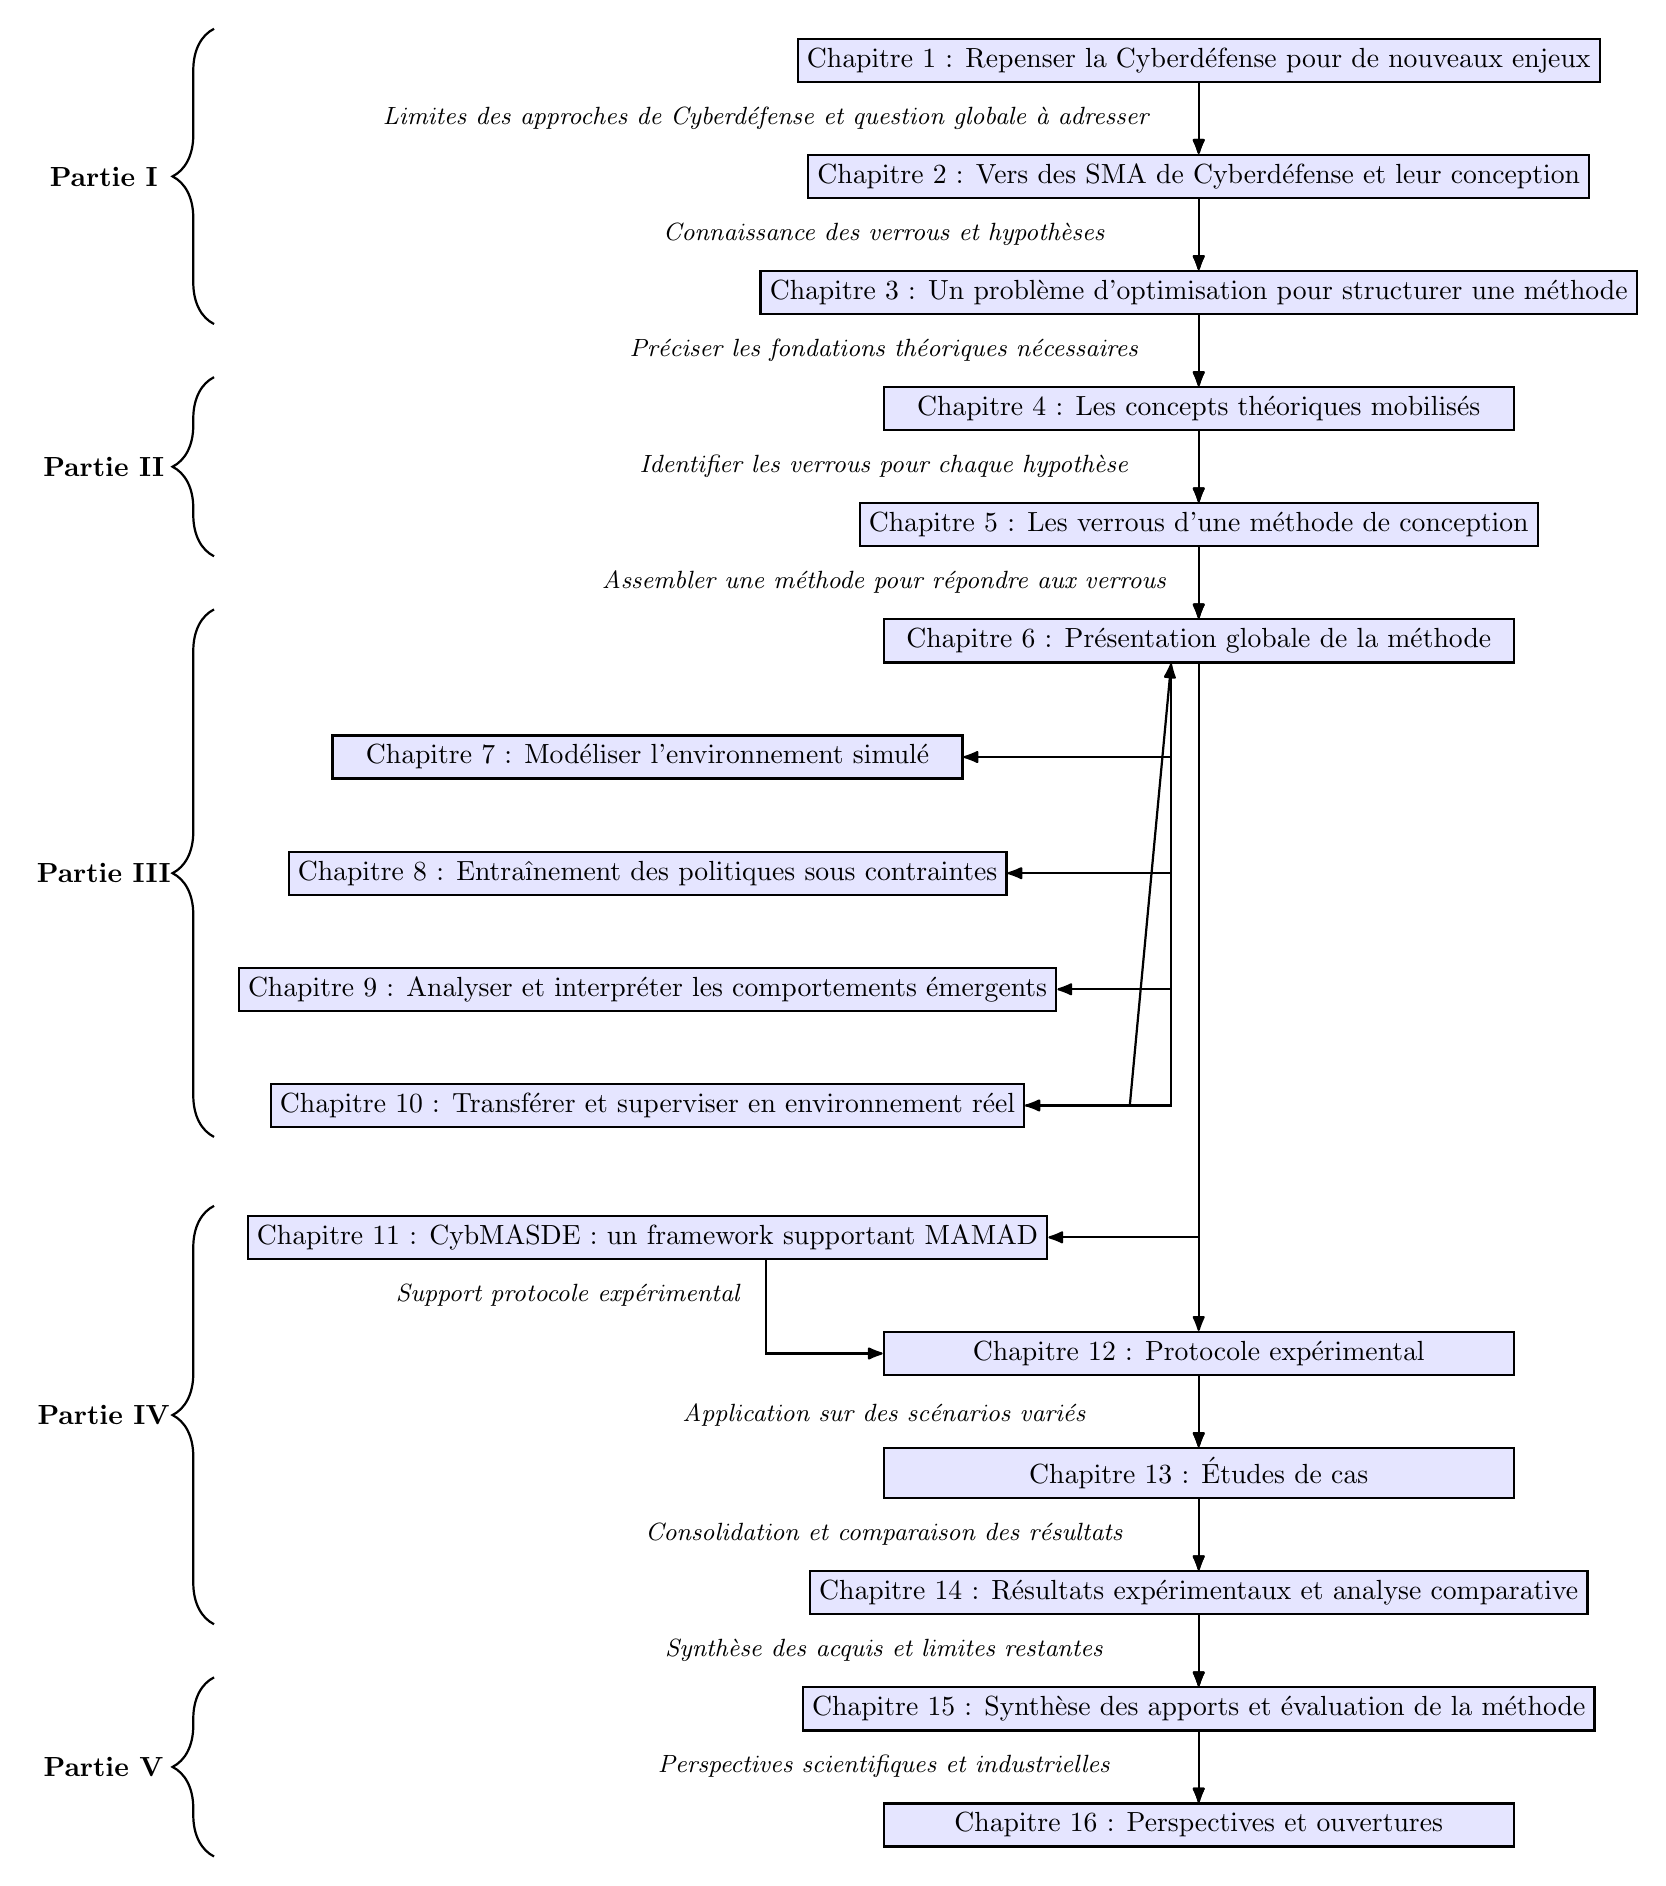
\begin{tikzpicture}[
    chapter/.style = {draw, thick, fill=blue!10, minimum width=8cm, align=left, font=\normalsize},
    arrow/.style = {-{Latex[round]}, thick},
    partlabel/.style = {rotate=90, font=\bfseries, align=center},
    dashedline/.style = {red, thick, dashed},
    node distance=0.9cm and 2cm,
    annotated/.style={above,font=\small\itshape, inner sep=1pt, yshift=5.5mm, xshift=-4cm}
    ]

    % Chapitres principaux (colonne verticale)
    \node[chapter] (c1) {Chapitre 1 : Repenser la Cyberdéfense pour de nouveaux enjeux};
    \node[chapter, below=of c1] (c2) {Chapitre 2 : Vers des SMA de Cyberdéfense et leur conception};
    \node[chapter, below=of c2] (c3) {Chapitre 3 : Un problème d'optimisation pour structurer une méthode};

    \node[chapter, below=of c3] (c4) {Chapitre 4 : Les concepts théoriques mobilisés};
    \node[chapter, below=of c4] (c5) {Chapitre 5 : Les verrous d'une méthode de conception};

    \node[chapter, below=of c5] (c6) {Chapitre 6 : Présentation globale de la méthode};

    % Flèches verticales principales avec annotations
    \draw[arrow] (c1) -- (c2) node[annotated, xshift=-1.5cm] {Limites des approches de Cyberdéfense et question globale à adresser};
    \draw[arrow] (c2) -- (c3) node[annotated] {Connaissance des verrous et hypothèses};
    \draw[arrow] (c3) -- (c4) node[annotated] {Préciser les fondations théoriques nécessaires};
    \draw[arrow] (c4) -- (c5) node[annotated] {Identifier les verrous pour chaque hypothèse};
    \draw[arrow] (c5) -- (c6) node[annotated] {Assembler une méthode pour répondre aux verrous};

    % Branche de droite (activités)
    \node[chapter, below= of c6, xshift=-7cm] (c7) {Chapitre 7 : Modéliser l'environnement simulé};
    \node[chapter, below=of c7] (c8) {Chapitre 8 : Entraînement des politiques sous contraintes};
    \node[chapter, below=of c8] (c9) {Chapitre 9 : Analyser et interpréter les comportements émergents};
    \node[chapter, below=of c9] (c10) {Chapitre 10 : Transférer et superviser en environnement réel};

    % Suite verticale
    \node[chapter, below=7cm of c6, xshift=-7cm] (c11) {Chapitre 11 : CybMASDE : un framework supportant MAMAD};
    \node[chapter, below=of c11, xshift=7cm] (c12) {Chapitre 12 : Protocole expérimental};
    \node[chapter, below=of c12] (c13) {Chapitre 13 : Études de cas};
    \node[chapter, below=of c13] (c14) {Chapitre 14 : Résultats expérimentaux et analyse comparative};
    \node[chapter, below=of c14] (c15) {Chapitre 15 : Synthèse des apports et évaluation de la méthode};

    \node[chapter, below=of c15] (c16) {Chapitre 16 : Perspectives et ouvertures};

    % Arrows
    \foreach \i/\j in {c1/c2, c2/c3, c3/c4, c4/c5, c5/c6, c12/c13, c13/c14, c14/c15, c15/c16}
    \draw[arrow] (\i) -- (\j);

    % Flèches horizontales depuis c6
    \foreach \dest in {c7, c8, c9, c10}
    \draw[arrow] ($ (c6.south) + (-0.35,0) $) -- ++(0,0) |- (\dest.east);

    \draw[arrow] (c10.east) -- ++(1.325,0) -- ($ (c6.south) + (-0.35,0) $);

    \draw[arrow] (c6.south) -- ++(0,0) |- (c11.east);

    \draw[arrow] ($ (c11.south) + (1.5, 0) $) -- ++(0,0) |- (c12.west) node[annotated] {Support protocole expérimental};

    \draw[arrow] (c6.south) -- (c12.north);


    % Flèches suite expérimentale
    \draw[arrow] (c12) -- (c13) node[annotated] {Application sur des scénarios variés};
    \draw[arrow] (c13) -- (c14) node[annotated] {Consolidation et comparaison des résultats};
    \draw[arrow] (c14) -- (c15) node[annotated] {Synthèse des acquis et limites restantes};
    \draw[arrow] (c15) -- (c16) node[annotated] {Perspectives scientifiques et industrielles};


    % Partie labels à gauche
    \draw[decorate, decoration={brace, amplitude=15pt}, thick]
    ($(c9.west |- c3.west)+(-0.3,-0.4)$) -- ($(c9.west |- c1.west)+(-0.3,0.4)$)
    node[midway,xshift=-1.4cm,rotate=0]{\textbf{Partie I}};

    \draw[decorate, decoration={brace, amplitude=15pt}, thick]
    ($(c9.west |- c5.west)+(-0.3,-0.4)$) -- ($(c9.west |- c4.west)+(-0.3,0.4)$)
    node[midway,xshift=-1.4cm,rotate=0]{\textbf{Partie II}};

    \draw[decorate, decoration={brace, amplitude=15pt}, thick]
    ($(c9.west |- c10.west)+(-0.3,-0.4)$) -- ($(c9.west |- c6.west)+(-0.3,0.4)$)
    node[midway,xshift=-1.4cm,rotate=0]{\textbf{Partie III}};

    \draw[decorate, decoration={brace, amplitude=15pt}, thick]
    ($(c9.west |- c14.west)+(-0.3,-0.4)$) -- ($(c9.west |- c11.west)+(-0.3,0.4)$)
    node[midway,xshift=-1.4cm,rotate=0]{\textbf{Partie IV}};

    \draw[decorate, decoration={brace, amplitude=15pt}, thick]
    ($(c9.west |- c16.west)+(-0.3,-0.4)$) -- ($(c9.west |- c15.west)+(-0.3,0.4)$)
    node[midway,xshift=-1.4cm,rotate=0]{\textbf{Partie V}};

  \end{tikzpicture}
}

    }
    \caption{Schéma de l'organisation du manuscrit}
    \label{fig:organisation_manuscrit}
\end{figure}

% =================================================================

\part{Fondements théoriques, revue de littérature et verrous}

\begin{figure}[h!]
    \centering
    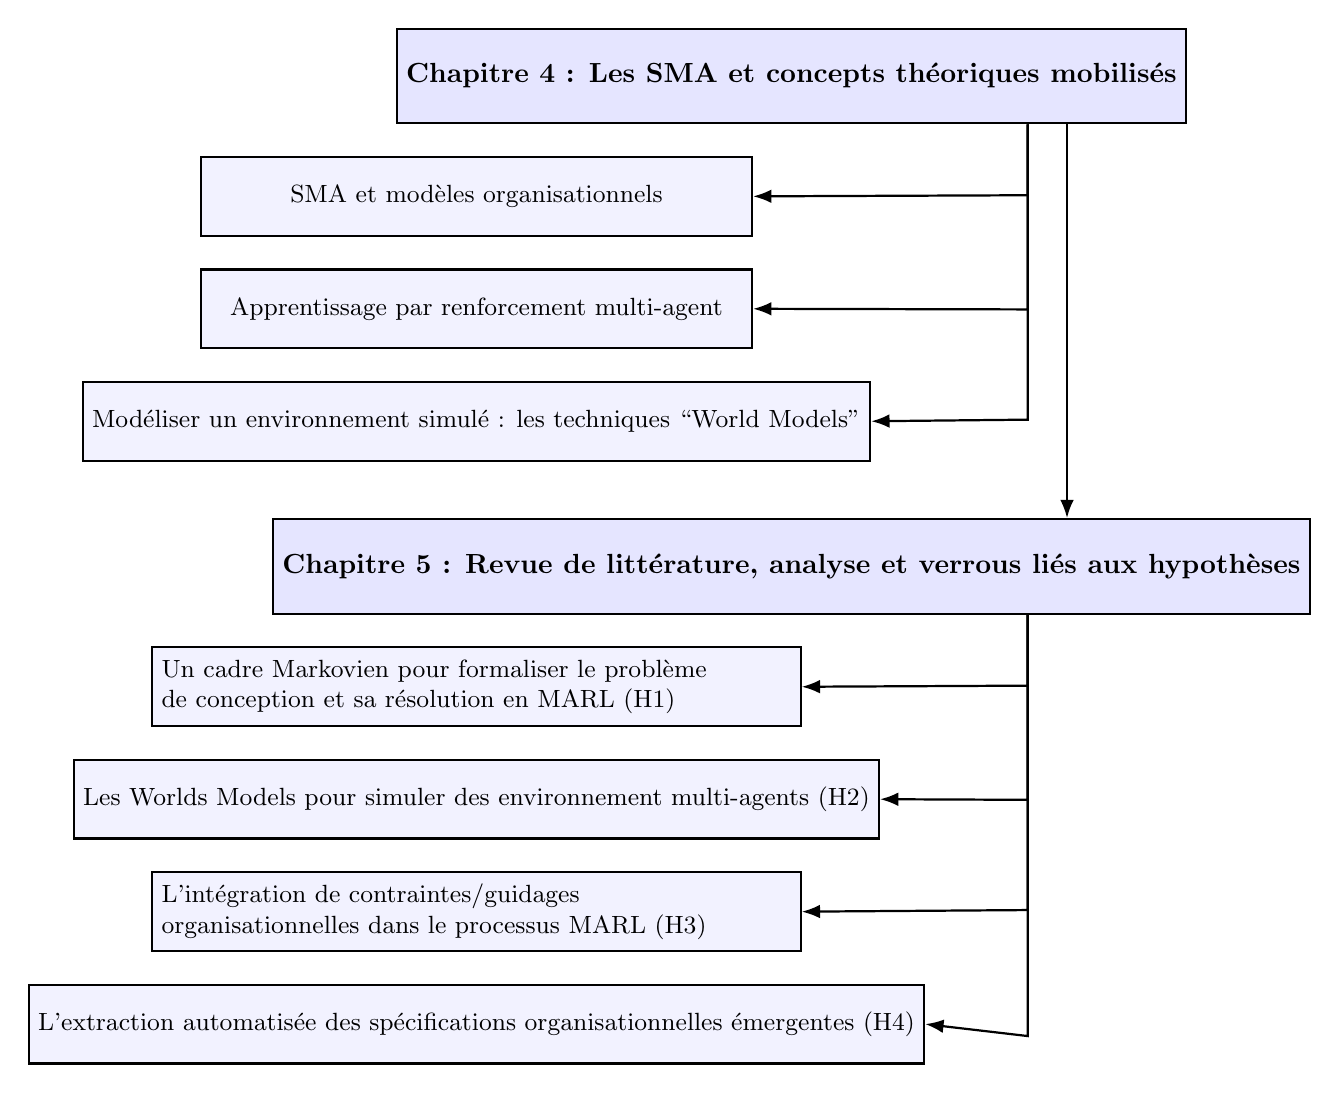
\begin{tikzpicture}[
    chapter/.style={draw, fill=blue!10, thick, minimum width=8cm, minimum height=1.2cm, text centered, font=\bfseries},
    section/.style={draw, fill=blue!5, thick, minimum width=7cm, minimum height=1cm, text centered, font=\small},
    arrow/.style={-Latex, thick},
    node distance=0.4cm
]

% Chapitre 4
\node[chapter] (ch4) {Chapitre 4 : Les SMA et concepts théoriques mobilisés};

\node[section, below=of ch4, xshift=-4cm] (ch4s1) {SMA et modèles organisationnels};
\node[section, below=of ch4s1] (ch4s2) {Apprentissage par renforcement multi-agent};
\node[section, below=of ch4s2] (ch4s3) {Modéliser un environnement simulé : les techniques \textquote{World Models}};

\draw[arrow] ($ (ch4.south) + (3,0) $) -- ++(0.,-0.9) -- (ch4s1.east);
\draw[arrow] ($ (ch4.south) + (3,0) $) -- ++(0.,-2.35) -- (ch4s2.east);
\draw[arrow] ($ (ch4.south) + (3,0) $) -- ++(0.,-3.75) -- (ch4s3.east);

% Chapitre 5
\node[chapter, below=5cm of ch4] (ch5) {Chapitre 5 : Revue de littérature, analyse et verrous liés aux hypothèses};

\node[section, below=of ch5, xshift=-4cm] (ch5s1) {\parbox{8cm}{Un cadre Markovien pour formaliser le problème \\ de conception et sa résolution en MARL (H1)}};
\node[section, below=of ch5s1] (ch5s2) {Les Worlds Models pour simuler des environnement multi-agents (H2)};
\node[section, below=of ch5s2] (ch5s3) {\parbox{8cm}{L'intégration de contraintes/guidages \\ organisationnelles dans le processus MARL (H3)}};
\node[section, below=of ch5s3] (ch5s4) {L'extraction automatisée des spécifications organisationnelles émergentes (H4)};

\draw[arrow] ($ (ch4.south) + (3.5,0) $) -- ($ (ch5.north) + (3.5,0) $);

\draw[arrow] ($ (ch5.south) + (3,0) $) -- ++(0.,-0.9) -- (ch5s1.east);
\draw[arrow] ($ (ch5.south) + (3,0) $) -- ++(0.,-2.35) -- (ch5s2.east);
\draw[arrow] ($ (ch5.south) + (3,0) $) -- ++(0.,-3.75) -- (ch5s3.east);
\draw[arrow] ($ (ch5.south) + (3,0) $) -- ++(0.,-5.35) -- (ch5s4.east);

\end{tikzpicture}

    \caption{Structure de la Partie II — Fondements théoriques, revue de littérature et verrous}
\end{figure}

\chapter{Concepts transversaux liés aux hypothèses}
% Objectif : définir les notions et modèles fondamentaux communs aux contributions.

\section{Systèmes Multi-Agents : coordination, rôles, interactions}
\section{Modèles organisationnels : MOISE+}

\section{Apprentissage par renforcement multi-agent (MARL)}

\section{Techniques \textquote{World Models}}

\chapter{Revue de littérature, analyse et verrous liés aux hypothèses}
% Objectif : pour chaque hypothèse H1-H5, analyser le domaine lié, identifier un manque, et formuler l'hypothèse comme réponse.

\section{H1 : Formalisation du problème (Dec-POMDP contraint)}
\section{H2 : Modélisation par apprentissage de l'environnement (World Models)}
\section{H3 : Résolution par MARL adaptatif}
\section{H4 : Guidage organisationnel via contraintes MOISE+ (OAC/TRF)}
\section{H5 : Analyse organisationnelle (rôles/objectifs émergents)}

\part{Méthode de conception : MAMAD}

\begin{figure}[h!]
    \centering
    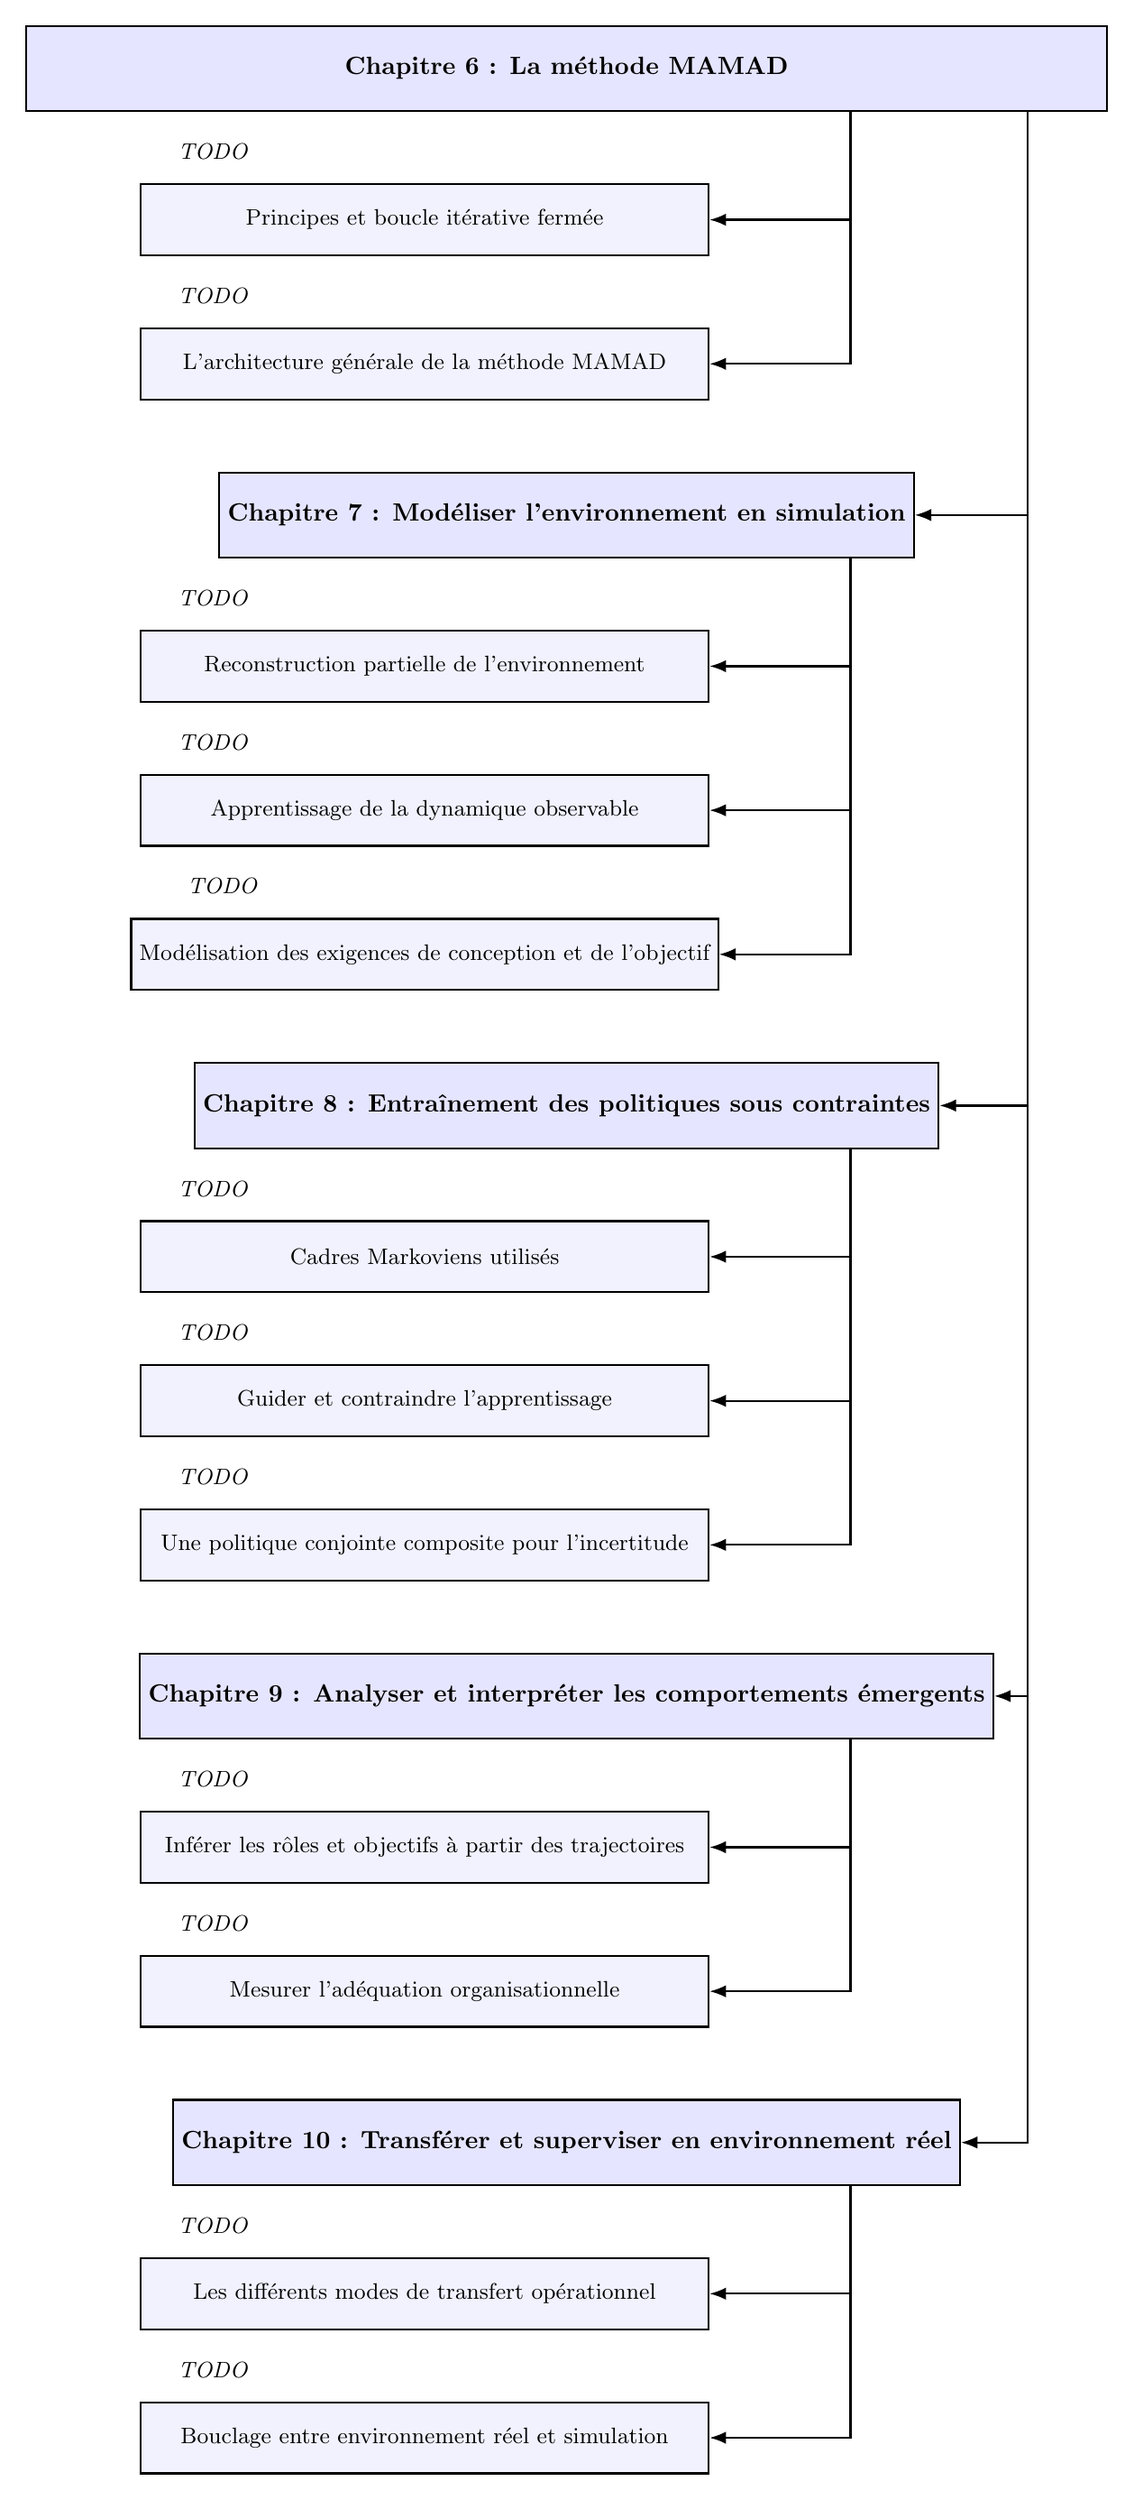
\begin{tikzpicture}[
    chapter/.style={draw, fill=blue!10, thick, minimum width=9cm, minimum height=1.2cm, text centered, font=\bfseries},
    section/.style={draw, fill=blue!5, thick, minimum width=8cm, minimum height=1cm, text centered, font=\small},
    arrow/.style={-Latex, thick},
    node distance=0.4cm,
    annotated/.style={above,font=\small\itshape, inner sep=1pt, yshift=0.8cm, xshift=-7cm}
]

% Chapitre 6 : MAMAD comme réponse
\node[chapter] (ch6) {\parbox{15cm}{\centering Chapitre 6 : La méthode MAMAD}};
\node[section, below=1cm of ch6, xshift=-2cm] (ch6s1) {Principes et boucle itérative fermée};
\node[section, below=1cm of ch6s1] (ch6s2) {L'architecture générale de la méthode MAMAD};

\draw[arrow] ($ (ch6.south) + (4.0,0) $) -- ++(0,0) |- (ch6s1.east) node[annotated] {TODO};
\draw[arrow] ($ (ch6.south) + (4.0,0) $) -- ++(0,0) |- (ch6s2.east) node[annotated] {TODO};

% Chapitre 7 : Phase 1 — Modélisation
\node[chapter, below=1cm of ch6s2, xshift=2cm] (ch7) {Chapitre 7 : Modéliser l'environnement en simulation};
\node[section, below=1cm of ch7, xshift=-2cm] (ch7s1) {Reconstruction partielle de l’environnement};
\node[section, below=1cm of ch7s1] (ch7s2) {Apprentissage de la dynamique observable};
\node[section, below=1cm of ch7s2] (ch7s3) {Modélisation des exigences de conception et de l'objectif};

\draw[arrow] ($ (ch7.south) + (4.0,0) $) -- ++(0,0) |- (ch7s1.east) node[annotated] {TODO};
\draw[arrow] ($ (ch7.south) + (4.0,0) $) -- ++(0,0) |- (ch7s2.east) node[annotated] {TODO};
\draw[arrow] ($ (ch7.south) + (4.0,0) $) -- ++(0,0) |- (ch7s3.east) node[annotated] {TODO};

% Chapitre 8 : Phase 2 — Apprentissage guidé
\node[chapter, below=1cm of ch7s3, xshift=2cm] (ch8) {Chapitre 8 : Entraînement des politiques sous contraintes};
\node[section, below=1cm of ch8, xshift=-2cm] (ch8s1) {Cadres Markoviens utilisés};
\node[section, below=1cm of ch8s1] (ch8s2) {Guider et contraindre l'apprentissage};
\node[section, below=1cm of ch8s2] (ch8s3) {Une politique conjointe composite pour l'incertitude};

\draw[arrow] ($ (ch8.south) + (4.0,0) $) -- ++(0,0) |- (ch8s1.east) node[annotated] {TODO};
\draw[arrow] ($ (ch8.south) + (4.0,0) $) -- ++(0,0) |- (ch8s2.east) node[annotated] {TODO};
\draw[arrow] ($ (ch8.south) + (4.0,0) $) -- ++(0,0) |- (ch8s3.east) node[annotated] {TODO};

% Chapitre 9 : Phase 3 — Analyse
\node[chapter, below=1cm of ch8s3, xshift=2cm] (ch9) {Chapitre 9 : Analyser et interpréter les comportements émergents};
\node[section, below=1cm of ch9, xshift=-2cm] (ch9s1) {Inférer les rôles et objectifs à partir des trajectoires};
\node[section, below=1cm of ch9s1] (ch9s2) {Mesurer l’adéquation organisationnelle};

\draw[arrow] ($ (ch9.south) + (4.0,0) $) -- ++(0,0) |- (ch9s1.east) node[annotated] {TODO};
\draw[arrow] ($ (ch9.south) + (4.0,0) $) -- ++(0,0) |- (ch9s2.east) node[annotated] {TODO};


% Chapitre 10 : Phase 4 — Transfert
\node[chapter, below=1cm of ch9s2, xshift=2cm] (ch10) {Chapitre 10 : Transférer et superviser en environnement réel};
\node[section, below=1cm of ch10, xshift=-2cm] (ch10s1) {Les différents modes de transfert opérationnel};
\node[section, below=1cm of ch10s1] (ch10s2) {Bouclage entre environnement réel et simulation};

\draw[arrow] ($ (ch10.south) + (4.0,0) $) -- ++(0,0) |- (ch10s1.east) node[annotated] {TODO};
\draw[arrow] ($ (ch10.south) + (4.0,0) $) -- ++(0,0) |- (ch10s2.east) node[annotated] {TODO};


\draw[arrow] ($ (ch6.south) + (6.5,0) $) -- ++(0,0) |- (ch7.east);
\draw[arrow] ($ (ch6.south) + (6.5,0) $) -- ++(0,0) |- (ch8.east);
\draw[arrow] ($ (ch6.south) + (6.5,0) $) -- ++(0,0) |- (ch9.east);
\draw[arrow] ($ (ch6.south) + (6.5,0) $) -- ++(0,0) |- (ch10.east);


\end{tikzpicture}

    \caption{Structure de la Partie III — Méthode de conception : MAMAD}
\end{figure}

\chapter{MAMAD comme réponse}

\section{Principe général et boucle itérative}

\section{Architecture globale}

\chapter{Phase 1 — Modélisation en simulation}
\section{Reconstruction partielle de l'environnement}
\section{Apprentissage de la dynamique observable}
\section{Intégration des contraintes de déploiement}

\chapter{Phase 2 — Apprentissage guidé/contraint}
\section{Cadres d'entraînement MARL utilisés}
\section{Contraintes organisationnelles dans MARL (OAC, TRF)}
\section{Politique composite et filtrage d'actions}

\chapter{Phase 3 — Analyse post-entraînement}
\section{Méthodes d'inférence des rôles et objectifs}
\section{Indicateurs : SOF, FOF, OF}
\section{Outil TEMM : fonctionnement, cas d'usage}

\chapter{Phase 4 — Transfert et supervision}
\section{Modes de transfert (centralisé/distribué)}
\section{Bouclage entre environnement réel et simulation}

\part{Cadre expérimental et analyse des résultats}

\begin{figure}[h!]
    \centering
    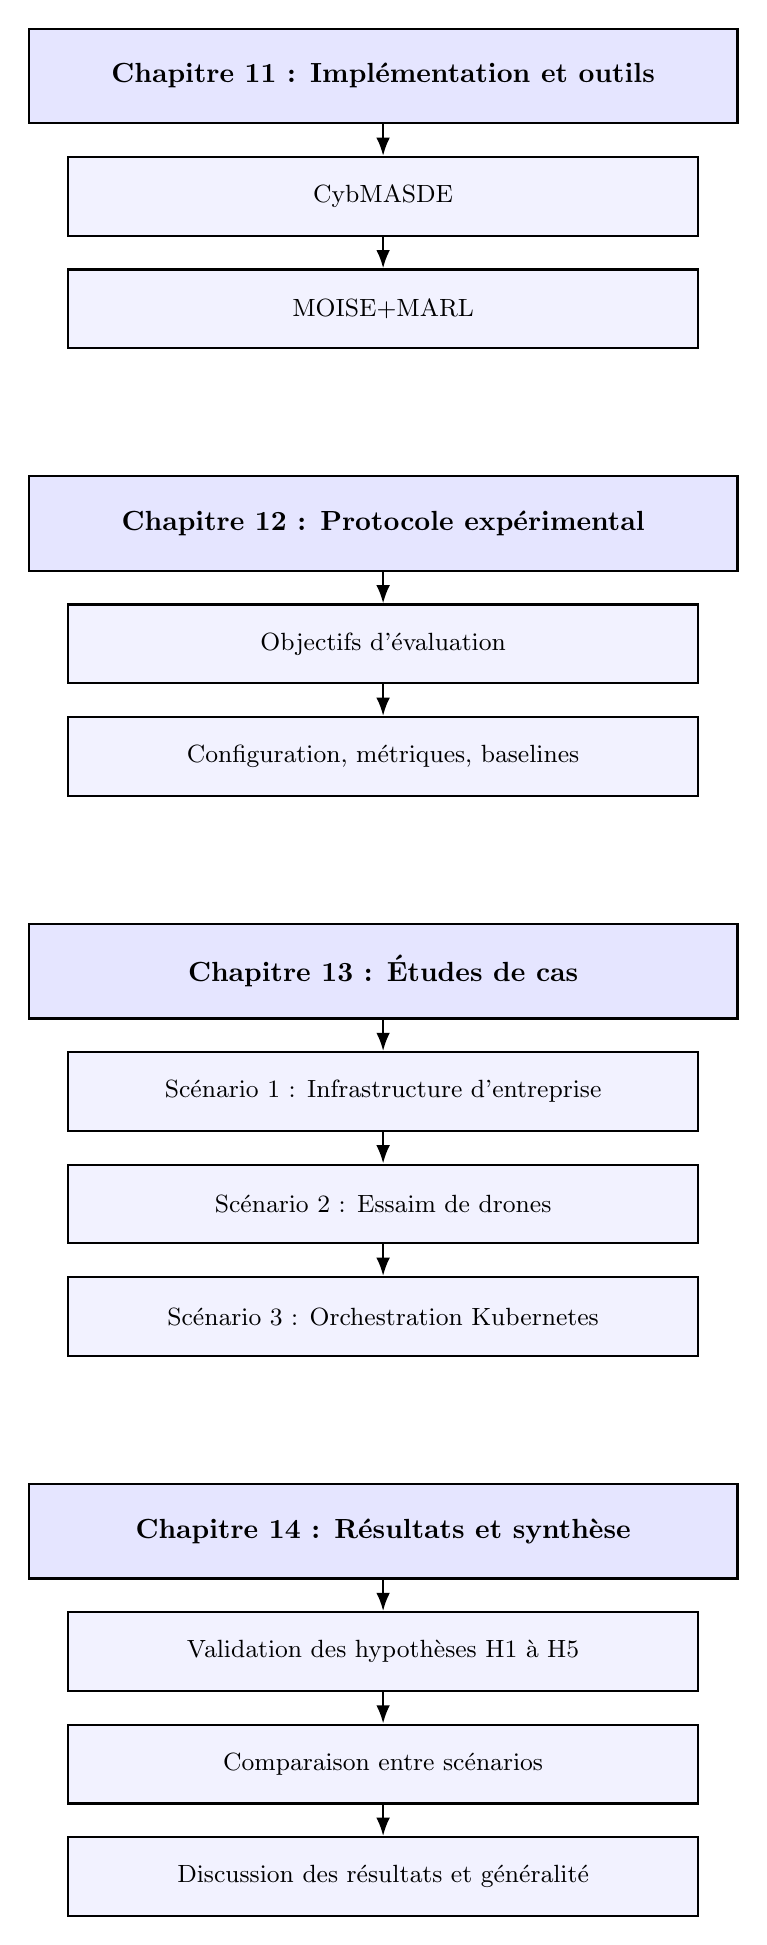
\begin{tikzpicture}[
    chapter/.style={draw, fill=blue!10, thick, minimum width=9cm, minimum height=1.2cm, text centered, font=\bfseries},
    section/.style={draw, fill=blue!5, thick, minimum width=8cm, minimum height=1cm, text centered, font=\small},
    arrow/.style={-Latex, thick},
    node distance=0.4cm
]

% Chapitre 11 : Implémentation et outils
\node[chapter] (ch11) {Chapitre 11 : Implémentation et outils};
\node[section, below=of ch11] (ch11s1) {CybMASDE};
\node[section, below=of ch11s1] (ch11s2) {MOISE+MARL};

\draw[arrow] (ch11) -- (ch11s1);
\draw[arrow] (ch11s1) -- (ch11s2);

% Chapitre 12 : Protocole expérimental
\node[chapter, below=1.6cm of ch11s2] (ch12) {Chapitre 12 : Protocole expérimental};
\node[section, below=of ch12] (ch12s1) {Objectifs d’évaluation};
\node[section, below=of ch12s1] (ch12s2) {Configuration, métriques, baselines};

\draw[arrow] (ch12) -- (ch12s1);
\draw[arrow] (ch12s1) -- (ch12s2);

% Chapitre 13 : Études de cas
\node[chapter, below=1.6cm of ch12s2] (ch13) {Chapitre 13 : Études de cas};
\node[section, below=of ch13] (ch13s1) {Scénario 1 : Infrastructure d’entreprise};
\node[section, below=of ch13s1] (ch13s2) {Scénario 2 : Essaim de drones};
\node[section, below=of ch13s2] (ch13s3) {Scénario 3 : Orchestration Kubernetes};

\draw[arrow] (ch13) -- (ch13s1);
\draw[arrow] (ch13s1) -- (ch13s2);
\draw[arrow] (ch13s2) -- (ch13s3);

% Chapitre 14 : Résultats et synthèse
\node[chapter, below=1.6cm of ch13s3] (ch14) {Chapitre 14 : Résultats et synthèse};
\node[section, below=of ch14] (ch14s1) {Validation des hypothèses H1 à H5};
\node[section, below=of ch14s1] (ch14s2) {Comparaison entre scénarios};
\node[section, below=of ch14s2] (ch14s3) {Discussion des résultats et généralité};

\draw[arrow] (ch14) -- (ch14s1);
\draw[arrow] (ch14s1) -- (ch14s2);
\draw[arrow] (ch14s2) -- (ch14s3);

\end{tikzpicture}

    \caption{Structure de la Partie IV — Cadre expérimental et analyse des résultats}
\end{figure}

\chapter{Implémentation et outils}
\section{CybMASDE}
\section{MOISE+MARL}

\chapter{Protocole expérimental}
\section{Objectifs d'évaluation}
\section{Configuration, métriques, baselines}

\chapter{Études de cas}
\section{Scénario 1 : Infrastructure d'entreprise}
\section{Scénario 2 : Essaim de drones}
\section{Scénario 3 : Orchestration Kubernetes}

\chapter{Résultats et synthèse}
\section{Validation des hypothèses H1 à H5}
\section{Comparaison entre scénarios}
\section{Discussion des résultats et généralité}

\part{Conclusion et perspectives}

\begin{figure}[h!]
    \centering
    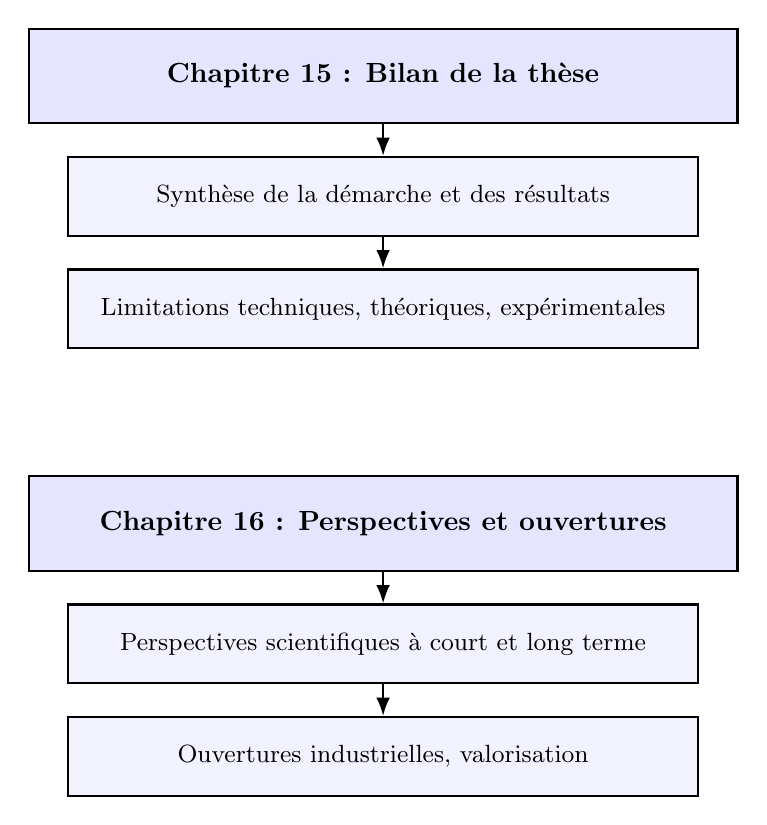
\begin{tikzpicture}[
    chapter/.style={draw, fill=blue!10, thick, minimum width=9cm, minimum height=1.2cm, text centered, font=\bfseries},
    section/.style={draw, fill=blue!5, thick, minimum width=8cm, minimum height=1cm, text centered, font=\small},
    arrow/.style={-Latex, thick},
    node distance=0.4cm
]

% Chapitre 15 : Bilan de la thèse
\node[chapter] (ch15) {Chapitre 15 : Bilan de la thèse};
\node[section, below=of ch15] (ch15s1) {Synthèse de la démarche et des résultats};
\node[section, below=of ch15s1] (ch15s2) {Limitations techniques, théoriques, expérimentales};

\draw[arrow] (ch15) -- (ch15s1);
\draw[arrow] (ch15s1) -- (ch15s2);

% Chapitre 16 : Perspectives et ouvertures
\node[chapter, below=1.6cm of ch15s2] (ch16) {Chapitre 16 : Perspectives et ouvertures};
\node[section, below=of ch16] (ch16s1) {Perspectives scientifiques à court et long terme};
\node[section, below=of ch16s1] (ch16s2) {Ouvertures industrielles, valorisation};

\draw[arrow] (ch16) -- (ch16s1);
\draw[arrow] (ch16s1) -- (ch16s2);

\end{tikzpicture}

    \caption{Structure de la Partie V — Conclusion et perspectives}
\end{figure}

\chapter{Bilan de la thèse}

\section{Synthèse de la démarche et des résultats}

\section{Limitations techniques, théoriques, expérimentales}

\chapter{Perspectives et ouvertures}
\section{Perspectives scientifiques à court et long terme}
\section{Ouvertures industrielles, valorisation}



%********************************************************************
% Other Stuff in the Back
%*******************************************************
\cleardoublepage\include{FrontBackmatter/Bibliography}
% \cleardoublepage\include{FrontBackmatter/Declaration}
% \cleardoublepage\include{FrontBackmatter/Colophon}

% ********************************************************************
% Backmatter
%*******************************************************
\appendix
%\renewcommand{\thechapter}{\alph{chapter}}
\cleardoublepage
% \part{Appendix}

%********************************************************************
% Appendix
%*******************************************************
% If problems with the headers: get headings in appendix etc. right
%\markboth{\spacedlowsmallcaps{Appendix}}{\spacedlowsmallcaps{Appendix}}
\chapter{Appendices}

\section{List of included papers}

\section{Experiments details}


\end{document}
% ********************************************************************
